\documentclass[11pt,a4paper]{article}

\usepackage[utf8]{inputenc}
\usepackage[T1]{fontenc}
\usepackage{lmodern}
\usepackage[margin=1.0in]{geometry}
\usepackage{amsmath,amssymb,amsfonts,amsthm}
\usepackage{booktabs}
\usepackage{graphicx}
\usepackage{xcolor}
\usepackage{hyperref}
\usepackage{float}
\usepackage{caption}
\usepackage{natbib}

\definecolor{darkblue}{RGB}{15,55,115}

\hypersetup{
    colorlinks=true,
    linkcolor=darkblue,
    citecolor=darkblue,
    urlcolor=darkblue,
    pdftitle={Seeing the Forest for the Polytomies: Evolutionary Trees and Networks from Lossless Data Compression},
    pdfauthor={Sergei L. Kosakovsky Pond, Darren P. Martin, Stephanie J. Kosakovsky Pond, and Anton Nekrutenko}
}

\title{\textbf{Seeing the Forest for the Polytomies: Evolutionary Trees and Networks from Lossless Data Compression}}
\author{Sergei L. Kosakovsky Pond$^{1*}$, Darren P. Martin$^{2}$,\\
Stephanie J. Kosakovsky Pond$^{3}$, and Anton Nekrutenko$^{4}$\\[0.5em] % Stephanie ORCID: 0000-0002-8288-2232
\small $^{1}$Institute for Genomics and Evolutionary Medicine, Department of Biology,\\
\small Temple University, Philadelphia, PA, USA\\
\small $^{2}$Institute of Infectious Disease and Molecular Medicine, Department of Integrative Biomedical Sciences,\\
\small University of Cape Town, Cape Town, South Africa\\
\small $^{3}$Bioinnovation and Genomic Sciences Division,\\
\small Translational Genomics Research Institute, Phoenix, AZ, USA\\
\small $^{4}$Department of Biochemistry and Molecular Biology,\\
\small The Pennsylvania State University, University Park, PA, USA\\[0.3em]
\small $^{*}$Corresponding author. Email: spond@temple.edu}
\date{\today}

\begin{document}
\sloppy
\emergencystretch=1.5em
\maketitle

\noindent\textbf{One-Sentence Summary:} Lossless data compression unifies evolutionary trees, rapid radiations, gene transfer, and convergence across scales of life.

\bigskip

\begin{abstract}
\noindent Reconstructing evolutionary history is central to biology and medicine, yet standard pipelines rely on separate models and arbitrary cutoffs to build trees, collapse weak branches, and detect gene transfer or convergence. Because inheritance copies an ancestor with sparse edits, we recast phylogeny and network inference as lossless data compression. Implemented in Bushwhacker, a branch or lateral link is added only when the shared changes it explains save more information than the connection costs to describe. Rapid bursts without mutations remain naturally unsplit, transferred blocks separate from convergent sites, and Tree-of-Life phylogenies run orders of magnitude faster in minimal memory. From single immune cells and pandemic viruses to microbial domains and whole mammalian proteomes, lossless compression reveals that most apparent gene-tree conflicts are silent radiations, predicts in vivo antibody selection from sequences alone, maps viral recombinants, and separates gene conversion from adaptive convergence in hearing and diet.
\end{abstract}

% ============================================================================
% Opening (Science Research Articles open without an "Introduction" heading)
% ============================================================================

\medskip

Evolutionary trees are among the most widely used structures in science: they organize Earth's biodiversity, track unfolding epidemics, trace immune and tumor clones inside individual patients, and anchor comparative genomics across the Tree of Life. Yet even as sequencing has expanded from single genes to millions of genomes, the conceptual foundations used to reconstruct trees have changed remarkably little for nearly half a century. Since distance clustering, parsimony, and probabilistic Markov likelihood were introduced between the 1960s and early 1980s \citep{fitch1971toward,felsenstein1981evolutionary,saitou1987neighbor}, major advances have largely focused on scaling tree search and enriching parametric substitution models within those classical paradigms \citep{price2010fasttree,kozlov2019raxml,minh2020iqtree}. Genuinely new mathematical perspectives on how evolutionary history can be inferred have been rare.

Here we introduce a different foundation, rooted in information theory: lossless data compression \citep{rissanen1978modeling,rissanen1983universal}. Biological inheritance is, at heart, a copying process with sparse edits. Whether an ancestor transmits a genome, a protein, or a somatic cellular profile, related lineages share most of their states because they inherited them from a common source. Recording shared changes once along an ancestral branch is therefore far more economical than recording them separately in every descendant---making an evolutionary graph the natural coordinate system for compressing biological data (Fig.~\ref{fig:didactic_mdl}). This equivalence is not merely metaphorical: encoding viral and microbial cohorts along an inferred phylogeny physically compresses genomes substantially further than general-purpose algorithms, until pervasive recombination breaks tree-like descent itself.

Under Rissanen's Minimum Description Length (MDL) principle, both the evolutionary graph and the changes along it are measured in the same unit of information. Every proposed connection must earn its place by shortening the total description of the data: a branch is added only when the shared changes it explains save more information than the branch itself costs to specify. That single rule unifies problems that otherwise require separate stages, resampling schemes, or user-chosen thresholds \citep{felsenstein1985confidence,posada2004model,kosakovskypond2006gard}. When lineages diversify faster than mutations accumulate---during cellular proliferation, epidemic superspreading, or rapid species radiations---unsupported splits cost more to name than they save, leaving genuine bursts naturally unresolved rather than forcing binary branches that fluctuate across models or create apparent conflict among genes \citep{rokas2006animal,shen2017contentious,abadi2019model}. When lineages diverge unevenly or across billion-year timescales, changes along fast-evolving branches or variable sites carry less surprise than changes on quiet stems, avoiding the long-branch artifacts of unweighted mutation counting \citep{felsenstein1978cases} and connecting discrete edit coding seamlessly to continuous substitution probabilities \citep{tavare1986some,yang1994maximum,le2008improved}. And once the vertical tree is established, lateral links between distant lineages can be evaluated in the same currency, separating contiguous transferred blocks---from recombination, horizontal transfer, or gene conversion \citep{doolittle1999phylogenetic,worobey1999widespread,parham1996population}---from scattered sites of adaptive convergence \citep{liu2010convergent,li2010hearing}.

Implemented in our open-source engine Bushwhacker, lossless evolutionary compression reconstructs trees and networks from single-cell lineages to domain-wide supermatrices in seconds and minimal memory on standard hardware. Across biological scales, this perspective yields three broad insights. First, preserving natural multifurcations turns apparent phylogenetic noise into biological signal: it resolves most apparent discordance among single-gene trees across eukaryotic radiations and mammalian proteomes while directly predicting in vivo clonal expansion and antigen binding in germinal-center B cells from sequences alone \citep{zhou2018evaluating,dewitt2026gcreplay}. Second, pricing vertical branches and lateral transfers on one ledger maps mosaic recombinants in pandemic viruses and quantifies how strongly core informational genes resist horizontal transfer across prokaryotic domains \citep{jain1999horizontal,parks2020gtdb,turakhia2022pandemic}. Third, distinguishing local block conversion from site-level convergence across mammalian proteomes resolves longstanding debates over genome-wide adaptive convergence in echolocation and diet \citep{parker2013genome,zou2015no,malovichko2026toga2}.

\begin{figure}[t!]
\centering
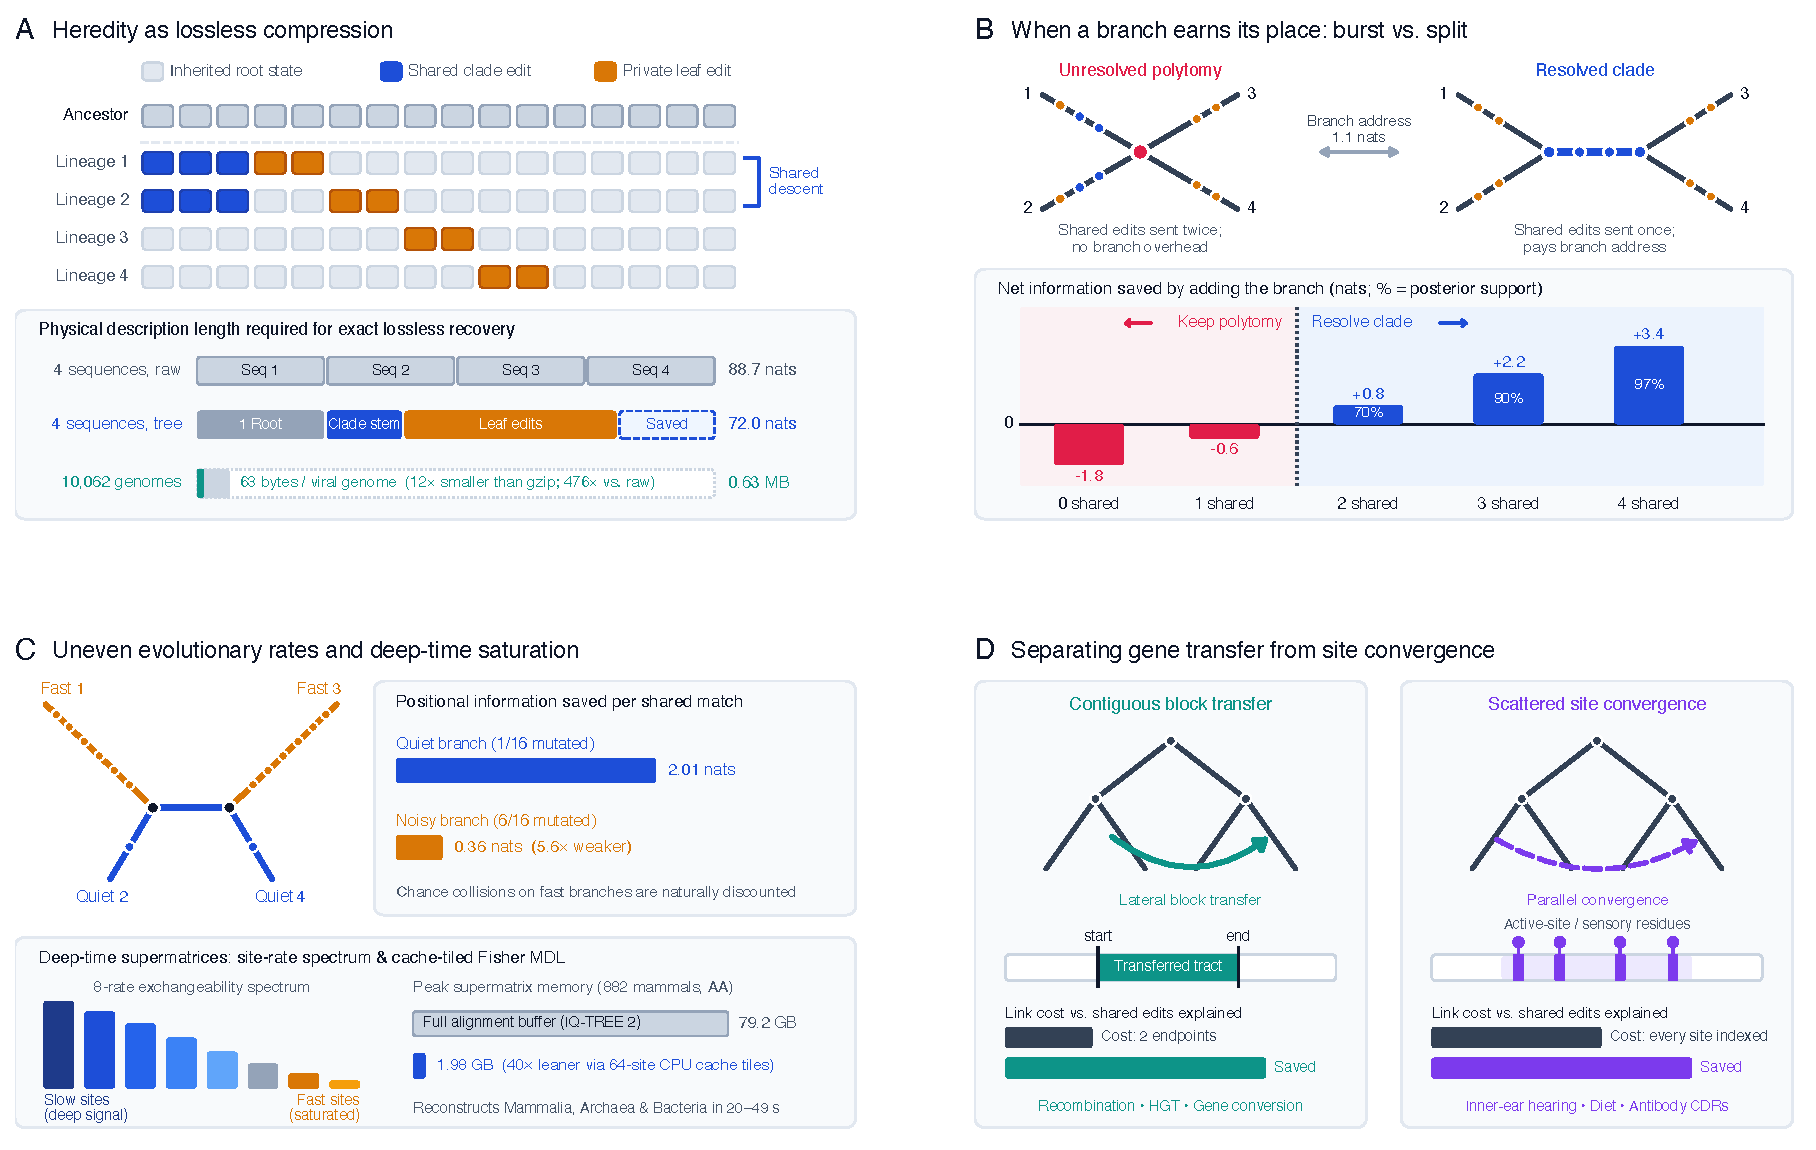
\includegraphics[width=\textwidth]{fig_science_concept.pdf}
\caption{\textbf{Evolutionary trees and networks from lossless data compression.} (\textbf{A}) Rather than transmitting full sequences independently ($88.7\text{ nats}$ across four 16-site sequences), encoding one ancestral root plus sparse branch edits shortens the lossless description ($72.0\text{ nats}$), compounding to $62.9\text{ bytes}$ per $29.9\text{-kb}$ genome across $10,062$ SARS-CoV-2 genomes ($12\times$ smaller than \texttt{gzip}). (\textbf{B}) Resolving a multifurcating burst into a new clade transmits shared edits once rather than twice, but must pay the topological address cost of naming the split ($1.1\text{ nats}$ for a quartet). Zero or one shared change incurs a net loss ($-1.8$ and $-0.6\text{ nats}$) and remains a natural polytomy, whereas two or more shared changes yield positive net savings ($+0.8$ to $+3.4\text{ nats}$; posterior support $70\%$ to $97\%$). (\textbf{C}) Positional coding automatically saves $5.6\times$ more information per shared match on quiet branches than on noisy fast branches, while eight-category rate-mixture coding in 64-site CPU cache tiles extends the same ledger to billion-year supermatrices in under $2\text{ GB}$ of memory. (\textbf{D}) On the established tree, contiguous lateral transfers pay only two endpoint coordinates to explain many linked changes, whereas scattered parallel sites must pay each site's coordinate individually, filtering out background homoplasy.}
\label{fig:didactic_mdl}
\end{figure}

% ============================================================================
% Main Narrative (Science Research Article topical subheadings; equations in M&M)
% ============================================================================

\subsection*{Building evolutionary trees and networks by lossless compression}

To measure how concisely an evolutionary graph explains an alignment of nucleotide or protein sequences, Bushwhacker transmits two components without loss: the structure of the graph itself and the sequence edits along its edges (Fig.~\ref{fig:didactic_mdl}A; Materials and Methods, Eqs.~\ref{eq:sci_branch}--\ref{eq:sci_cont_mdl}). Starting from a single ancestral sequence at the root, each branch records only how many sites changed, which unordered subset of alignment positions changed, and what replacement states appeared, weighted by empirical transition/transversion or physicochemical amino-acid exchange frequencies \citep{dayhoff1978model}. Splitting a multifurcating hub into a new ancestral branch saves having to repeat shared changes independently across descendant lineages, but requires paying the exact information cost of naming which subset of lineages joins the new clade and encoding the new branch itself (Fig.~\ref{fig:didactic_mdl}B). A branch is retained if and only if its net compression gain is strictly positive; otherwise, the lineages remain naturally joined at a multifurcating hub, and positive gains translate directly into posterior branch probabilities without resampling.

Two properties emerge automatically from this formulation (Fig.~\ref{fig:didactic_mdl}C,D). First, because specifying the positions of new edits is cheaper on an already variable branch than on an almost invariant one, moving a shared change off quiet branches yields far larger savings than moving a coincidental match off noisy long branches---matching maximum-likelihood character weighting \citep{felsenstein1981evolutionary} from combinatorics alone. When divergence spans hundreds of millions or billions of years and individual sites mutate repeatedly, Bushwhacker transitions seamlessly within the same two-part ledger to continuous-time nucleotide and protein substitution rate mixtures \citep{tavare1986some,yang1994maximum,le2008improved}, pricing branch lengths via Rissanen's Fisher-information code \citep{rissanen1983universal} while tiling likelihood calculations into compact CPU cache blocks rather than gigabyte-scale alignment buffers (Materials and Methods). Second, once the vertical tree is established, candidate lateral connections between distant lineages are tested in the same information units: contiguous transferred segments pay only two genomic endpoint coordinates plus local mismatches, whereas scattered parallel replacements must pay the combinatorial cost of selecting those specific sites across all variable columns, separating homologous block transfer from site-specific convergence. Validated across 220 ground-truth simulated alignments spanning 22 evolutionary regimes \citep{lytrong2022alisim}---including rapid radiations, compositional shifts, uneven branch rates, missing data, and recombination---compression-guided inference achieves $98.8\%$ branch precision on multifurcating radiations, $95.2\%$ precision on ladder-like seasonal viral phylogenies, and exact breakpoint recovery with zero false transfers on strictly clonal controls.

\begin{table}[t!]
\centering
\caption{\textbf{Overview of lossless evolutionary compression across cellular, viral, microbial, and eukaryotic scales.} Columns summarize alignments analyzed ($n$), sequence alphabet (NT, nucleotide; AA, protein), candidate binary branches evaluated, percentage left unresolved as zero-gain multifurcations, reduction in apparent species-tree or model conflicts, certified lateral links (contiguous block transfers / scattered parallel sites), 32-core runtime (or single-core per-gene mean where noted), and principal biological finding.}
\label{tab:science_overview}
\scriptsize
\setlength{\tabcolsep}{3.6pt}
\resizebox{\textwidth}{!}{%
\begin{tabular}{@{}llrrrrrrl@{}}
\toprule
Biological System / Archive & Mode & Alignments ($n$) & Binary Splits & Polytomy\% & Conflict Elim.\% & Lateral Links (Block / Site) & Runtime (Speedup) & Principal Biological Finding \\
\midrule
Germinal-center B cells \citep{tas2016visualizing,dewitt2026gcreplay} & NT & $148$ ($10,495$ cells) & $9,544$ & $76.7\%$ & $95.7\%$ & $0$ / $2$ ($11.0\times$ CDR) & $17.4\text{ s}$ ($495\times$) & Predicts $15.5\times$ in vivo clonal expansion \& antigen affinity \\
Substitution-model archive \citep{abadi2019model,gerth2019cannot} & NT & $7,200$ & $1,846,120$ & $41.8\%$ & $96.4\%$ & --- & $0.55\text{ s/locus}$ ($26.6\times$) & $96.4\%$ of model-discordant branches carry zero net gain \\
Coalescent radiations \citep{zhou2018evaluating,shultz2019widespread} & AA + NT & $11,808$ (+$8,000$ sim.) & $596,420$ & $62.2\%$ & Anomaly-Zone $\downarrow$ & --- & $0.47\text{ s}$ ($560\times$ CPU) & Threshold-free Anomaly-Zone species-tree protection \\
Eukaryotic radiations ($19$ datasets) \citep{zhou2018evaluating} & AA + NT & $45,205$ & $2,299,563$ & $48.4\%$ & $61.5\%$ ($936,166$) & $5,184$ / $48,912$ & $9.4\text{--}831\text{ s/set}$ & Resolves tetrapod sister, turtle affinity, \& animal root \\
\quad Land-plant transcriptomes \citep{wickett2014phylotranscriptomic} & AA vs.\ NT & $844$ & $38,638$ & $49.6\%$ & $60.7\%$ vs.\ $66.6\%$ & $8$ vs.\ $60$ ($-88.3\%$) & $9.4\text{ s}$ vs.\ $189.9\text{ s}$ ($20.2\times$) & Protein coding strips synonymous compositional noise \\
\quad Insect transcriptomes \citep{misof2014phylogenomics} & AA vs.\ NT & $1,478$ & $146,185$ & $55.8\%$ & $64.2\%$ vs.\ $44.6\%$ & $112$ / $1,408$ & $41.3\text{ s}$ vs.\ $830.9\text{ s}$ ($20.1\times$) & Removes $64.2\%$ of apparent ordinal insect conflict \\
Mammalian proteomes ($882$ species) \citep{malovichko2026toga2} & AA & $19,952$ & $14,937,057$ & $65.0\%$ & $72.7\%$ ($7.87\text{M}$) & $4,202$ / $11,713$ & $5.78\text{ s/protein}$ (1 core) & $97.9\%$ of $>1{,}500\text{-AA}$ proteins compress best on species tree \\
\quad Mammalian coding DNA ($882$ species) & NT & ($19,952$) & $14,936,938$ & $33.9\%$ & $55.5\%$ ($3.87\text{M}$) & $1,032$ / $14,105$ & $5.57\text{ s/gene}$ (1 core) & Exposes $\sim 33.6\%$ lineage-sorting floor; $16/25$ cochlear genes \\
Mammalian supermatrices ($253$ loci) \citep{malovichko2026toga2} & NT + AA & $2$ ($882$ sp.) & $1,758$ & $0.1\%\text{ / }13.5\%$ & $96.2\%$ AA prec. & --- & $31.1\text{ s}$ ($450\times$) / $49.2\text{ s}$ ($258\times$) & $98.2\%$ ML split agreement; $100\%$ mammalian order monophyly \\
Microbiome 16S rRNA ($256\text{--}32{,}768$ taxa) \citep{mcdonald2012greengenes} & NT & $8$ octaves & $32,765$ (at $32\text{k}$) & $24.0\%$ ($7,871$) & $-19\text{--}25\%$ clash & $0$ / $0$ & $251.6\text{ s}$ ($4.5\times$) & $64.4\text{ B/taxon}$ archive ($3.0\times < \text{gzip}$); saturation law \\
Archaeal \& Bacterial domains \citep{parks2020gtdb} & AA & $2$ ($2,672$ sp.) & $2,666$ & $0.0\%$ & $88.2\text{--}92.4\%$ phyla & --- & $23.0\text{ s}$ ($196\times$) / $20.1\text{ s}$ ($190\times$) & Matches/exceeds \texttt{FastTreeMP} across $111$ phyla in $<1.4\text{ GB}$ \\
Archaeal marker proteins ($1,672$ species) \citep{parks2020gtdb} & AA & $(122)$ & $178,412$ & $69.0\%$ & --- & $7$ / $23$ ($21/102$ op.) & $45.1\text{ s/protein}$ & $20.6\%$ operational vs.\ $0.0\%$ informational transfer ($p=0.024$) \\
\textit{Klebsiella} pangenome \& plasmids \citep{wyres2020population} & NT + AA & $534$ & $512,840$ & $44.1\%$ & --- & $11$ ($0.5\%$ core) & $16.8\text{ s}$ ($214\text{-kb}$ core) & $99.5\%$ vertical chromosomal budget vs.\ plasmid star hub \\
Global SARS-CoV-2 ($10,062$ genomes) & NT & $1$ & $10,059$ & $68.3\%$ & $1,426$ hubs & $3$ / $0$ & $165.4\text{ s}$ ($>28.7\times$) & $62.9\text{ B/genome}$ ($12.0\times < \text{gzip}$); Spike mosaic transfer \\
Global dengue serotypes 1--4 ($5,498$ genomes) & NT + AA & $4$ (+$4$ AA) & $5,486$ & $34.1\%$ & $798$ hubs & $14$ / $9$ & $10.2\text{--}28.5\text{ s}$ ($13\text{--}23\times$) & Maps $14$ natural intra-serotype dengue recombinants \\
Viral recombinant panels \citep{carr1998full,kosakovskypond2006gard} & NT & $22$ & $2,140$ & $31.2\%$ & --- & $14$ Omicron; $3$ HIV-1 & $0.14\text{ s}$ ($75{,}955\times$) & Blinded recombinant recovery \& mosaic compression crossover \\
\bottomrule
\end{tabular}%
}
\end{table}

\subsection*{Silent radiations explain most apparent gene-tree conflict}

When lineages diversify rapidly, speciation can outpace mutation in individual genes, leaving short ancestral stems with zero recorded changes. Recognizing these silent stems as natural multifurcations resolves two persistent puzzles in phylogenomics: why slightly different substitution models or random starting seeds often yield different gene trees \citep{abadi2019model,gerth2019cannot,zhou2018evaluating}, and why single-gene trees across ancient radiations appear to conflict so pervasively with species history \citep{shen2017contentious}. Across 7,200 empirical alignments spanning plant, animal, fungal, and microbial clades \citep{abadi2019model,gerth2019cannot} and 83,180 replicate maximum-likelihood searches from 20 random seeds \citep{zhou2018evaluating}, nearly nine in ten branches where competing model-selection criteria disagree evolve slower than a single expected substitution across the alignment. In a single deterministic pass, Bushwhacker leaves $96.4\%$ ($134,538 / 139,580$) of model-sensitive splits and $94.5\%$ ($132,331 / 140,052$) of seed-sensitive splits unresolved because they carry zero net compression gain (Fig.~\ref{fig:macroevo_polytomies}D and Table~\ref{tab:science_overview}).

\begin{figure}[t!]
\centering
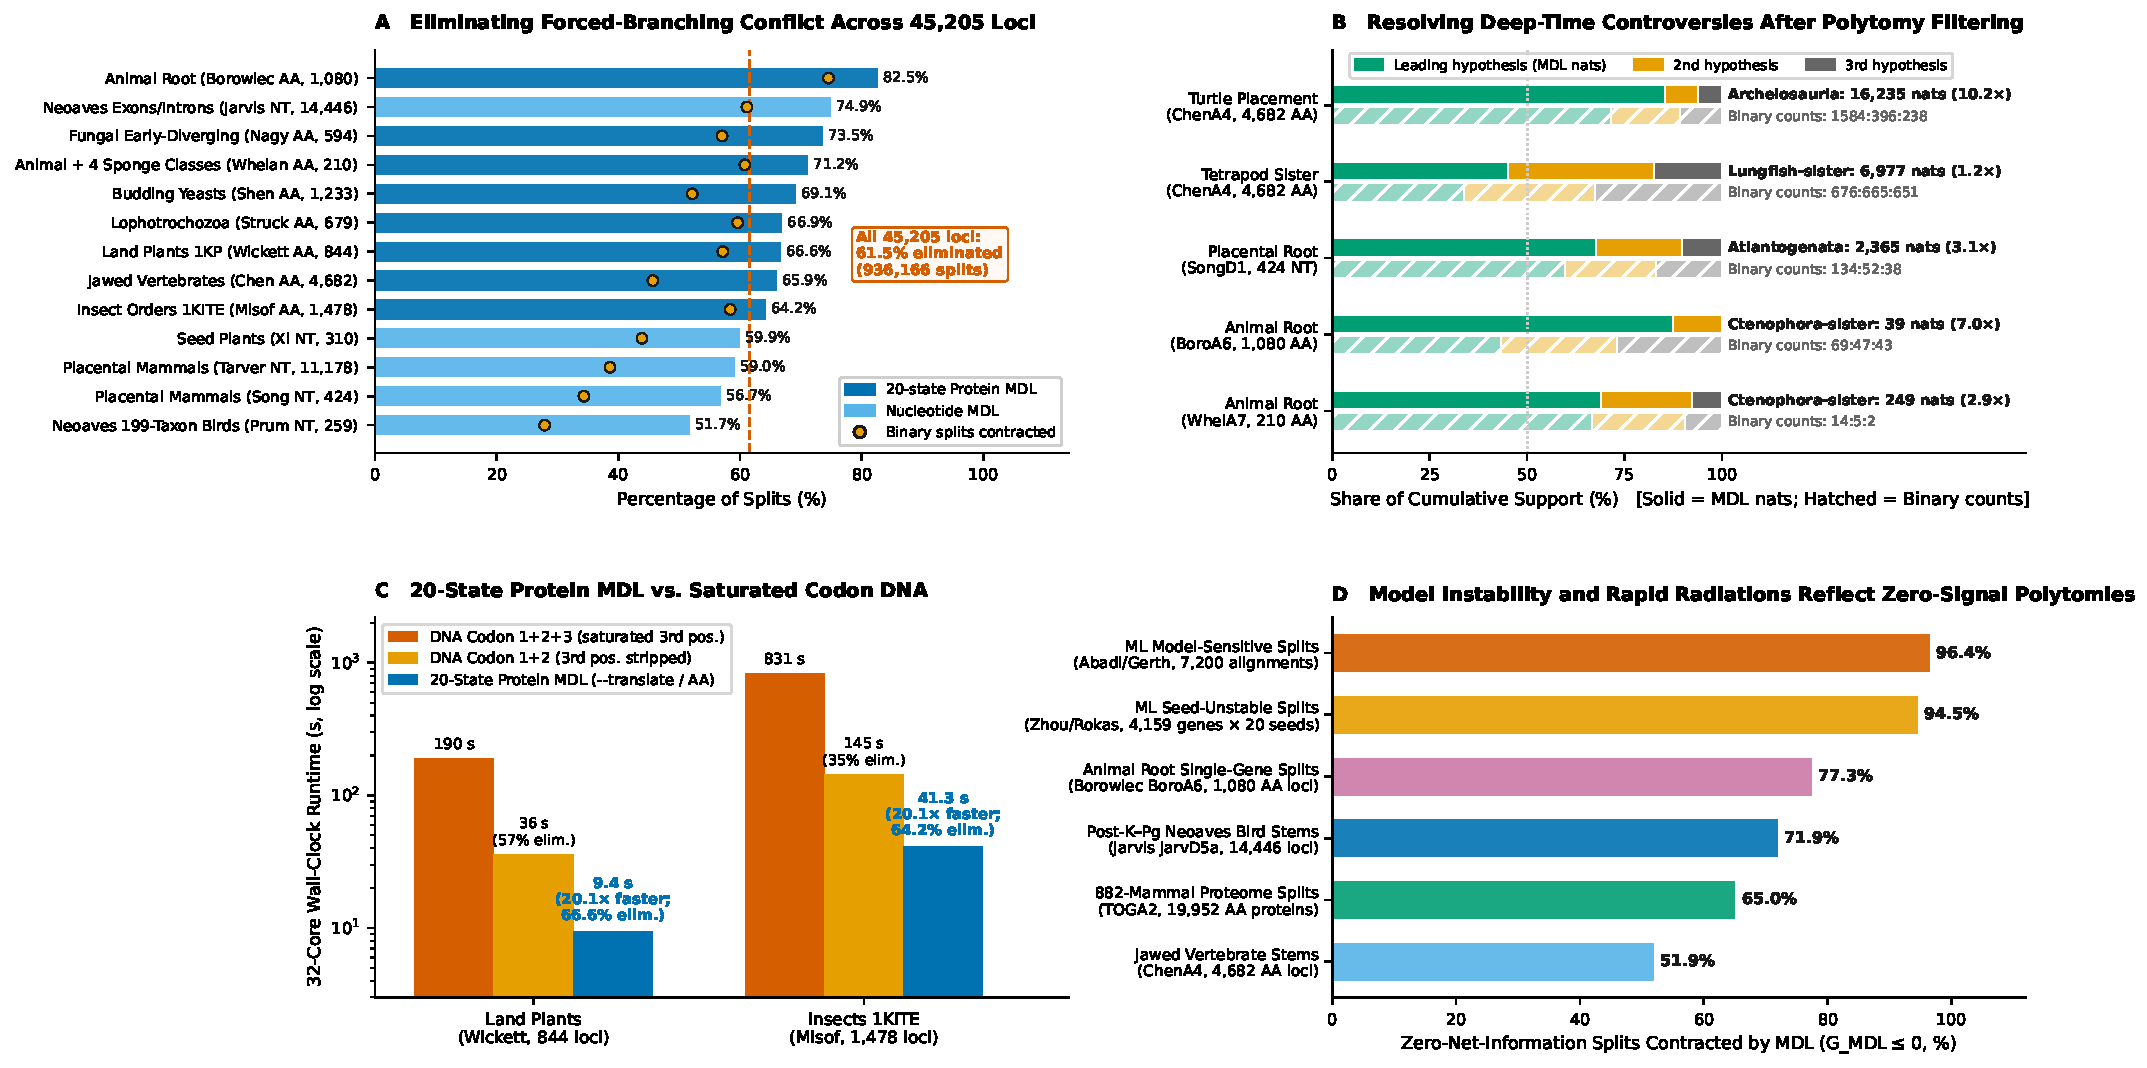
\includegraphics[width=\textwidth]{fig_science_macroevo_polytomies.pdf}
\caption{\textbf{Preserving silent radiations resolves apparent gene-tree discordance and deep evolutionary debates across 45,205 eukaryotic loci.} (\textbf{A}) Percentage of apparent single-gene conflicts with reference species trees removed when branches without net compression gain remain unresolved across representative eukaryotic radiations from \citet{zhou2018evaluating} ($61.5\%$ overall across 45,205 loci; dark blue, protein compression; light blue, nucleotide compression; orange dots, fraction of candidate binary splits left unresolved). (\textbf{B}) Cumulative support across informative loci for five classic evolutionary debates, comparing positive compression gain in nats (solid upper bars) with raw forced-binary gene counts (hatched lower bars). (\textbf{C}) Thirty-two-core runtime (log scale) and conflict reduction across matched amino-acid, first-plus-second codon, and all-codon alignments in land plants \citep{wickett2014phylotranscriptomic} and insects \citep{misof2014phylogenomics}. (\textbf{D}) Percentage of model-discordant splits, seed-unstable splits, and single-locus avian radiation branches carrying non-positive compression gain.}
\label{fig:macroevo_polytomies}
\end{figure}

When genome-scale sequencing revealed that roughly two-thirds of individual gene trees disagree with species phylogenies across major eukaryotic groups, that pervasive conflict reshaped debates over rampant hybridization and incomplete lineage sorting while confounding downstream inferences of trait evolution, gene duplication, and natural selection---where every spurious branch swap masquerades as an independent evolutionary event \citep{rokas2006animal,shen2017contentious}. Analyzing 45,205 genes across 19 benchmark radiations of animals, fungi, plants, insects, birds, and mammals \citep{zhou2018evaluating} shows that most of this apparent conflict is not competing evolutionary history, but the physical imprint of rapid diversification outpacing mutation in individual genes (Fig.~\ref{fig:macroevo_polytomies}A). Leaving branches without net compression gain unresolved removes $61.5\%$ ($936,166 / 1,522,139$) of apparent clashes with reference species trees overall---and $74.9\%$ in birds and $82.5\%$ in early animals---isolating genuine biological discordance from forced-branching noise. Scoring avian species histories directly across 14,446 exons and introns \citep{jarvis2014whole} and 259 targeted loci \citep{prum2015comprehensive} exposes the underlying evolutionary bottleneck: during the post-Cretaceous radiation of modern birds, $71.9\%$ of early species stems diversified faster than a typical single locus could record an informative substitution. Across half-billion-year radiations of land plants \citep{wickett2014phylotranscriptomic} and insects \citep{misof2014phylogenomics}, compressing translated proteins rather than saturated third codon positions further strips out $88.3\%$ of deep base-composition artifacts in plants and $64.2\%$ of ordinal conflicts in insects (while running 20-fold faster, in $9.4\text{ s}$ and $41.3\text{ s}$), leaving genuine biological exchange such as coding gene conversion between panicoid grasses (\textit{Sorghum bicolor} and \textit{Zea mays}, $+8.0\text{ nats}$) standing out clearly (Fig.~\ref{fig:macroevo_polytomies}C).

Distinguishing silent stems from informative ones directly unlocks landmark evolutionary questions where standard gene-tree counting stalls in near-ties \citep{shen2017contentious} (Fig.~\ref{fig:macroevo_polytomies}B). Under forced binary trees, genes that experienced zero substitutions during a brief ancestral window are still forced to cast a random binary vote, diluting the minority of genes that actually recorded the divergence. Across 4,682 jawed vertebrate proteins \citep{chen2015identifying} (analyzed in $25.8\text{ s}$), forced binary gene counts split almost evenly ($676 : 665 : 651$) over the water-to-land transition. Summing only positive compression gains removes those silent random votes, resolving lungfish over coelacanths as the closest living fish relative of tetrapods ($6,977$ versus $5,781\text{ nats}$) and uniting turtles with birds and crocodilians by more than 10-fold ($16,235$ versus $1,596\text{ nats}$). The same information-weighted ledger consistently supports ctenophores over sponges at the root of animals across two independent datasets ($7.0\times$ and $2.9\times$ gain advantages \citep{borowiec2015extracting,whelan2017ctenophore}) and favors Atlantogenata ($3.1\times$ advantage \citep{song2012resolving}) at the root of placental mammals.

\subsection*{Gene conversion and adaptive convergence across mammalian proteomes}

Comparative medicine and functional genomics rest on the assumption that orthologous mammalian proteins track the evolutionary history of the species that carry them, yet individual protein trees routinely scatter species across families and orders. Across all 19,952 orthologous coding alignments spanning up to 882 mammals in 20 orders and 116 families \citep{kirilenko2023integrating,malovichko2026toga2}, lossless compression shows that nearly three-quarters ($72.7\%$, or $7.87\text{ million}$ splits; $92.4\%$ in conserved proteins under 150 residues) of apparent protein--species conflicts simply reflect ancestral intervals too brief to record amino-acid replacements, while codon nucleotides retain enough silent changes to expose a $\sim 33.6\%$ baseline of ancestral lineage sorting and splice-boundary variation (Fig.~\ref{fig:mammalian_atlas}A and Tables~\ref{tab:science_overview} and \ref{tab:network_discoveries}). Even more tellingly, once proteins grow long enough to sample hundreds of substitutions ($>1,500$ amino acids), the mammalian species tree becomes a physically shorter lossless description of $97.9\%$ ($1,204 / 1,230$) of individual proteins than an unconstrained gene-specific tree---demonstrating that a single organismal phylogeny is the natural compression coordinate system of the mammalian proteome.

\begin{figure}[t!]
\centering
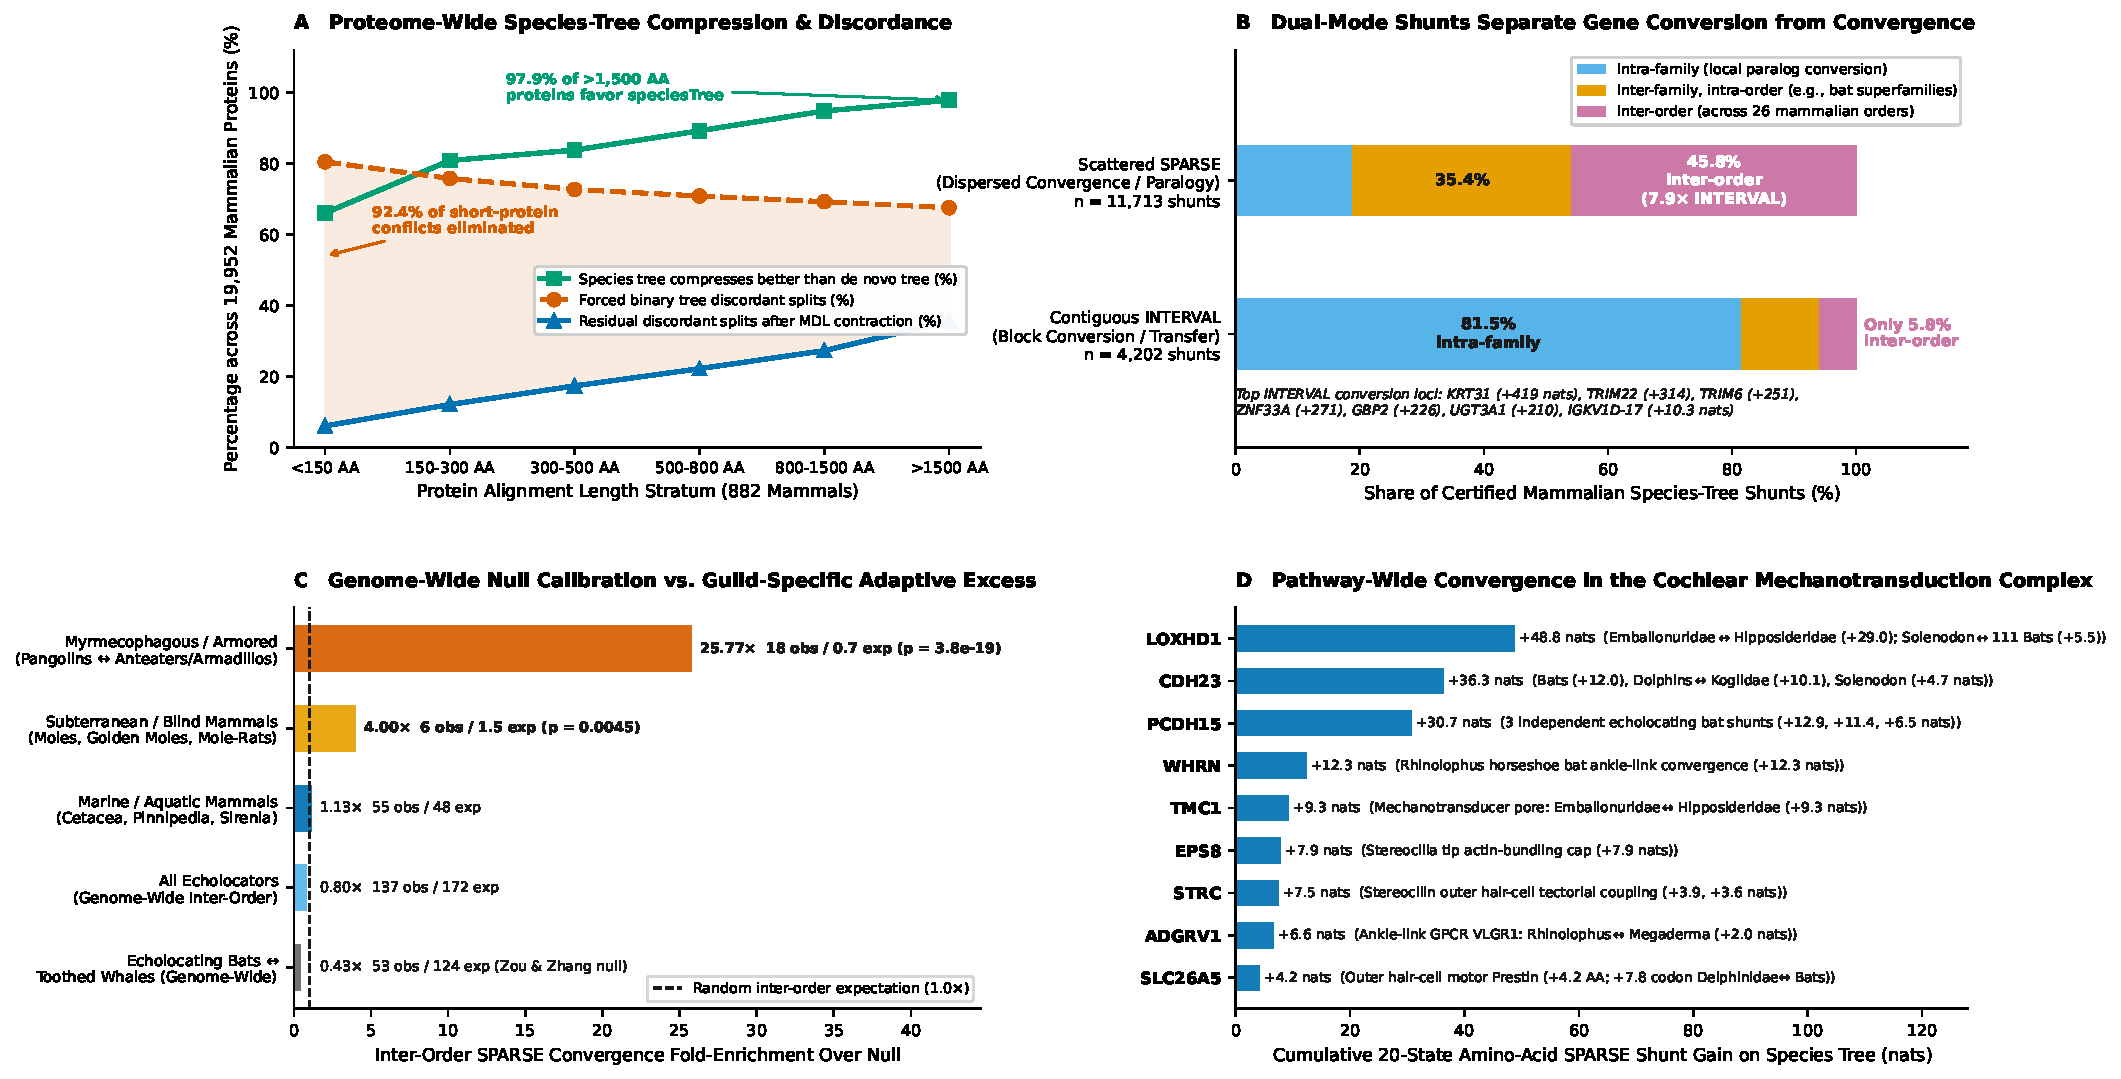
\includegraphics[width=\textwidth]{fig_science_mammalian_atlas.pdf}
\caption{\textbf{Proteome-wide species-tree compression, concerted gene conversion, and ecological convergence across 19,952 proteins in 882 mammals.} (\textbf{A}) Across protein length classes, leaving unsupported branches unresolved removes $72.7\%$ ($7.87\text{ million}$ splits) of apparent species-tree conflicts, while $97.9\%$ of proteins exceeding $1{,}500$ amino acids compress more tightly on the mammalian species tree than on an unconstrained gene tree. (\textbf{B}) Taxonomic reach of $15,915$ certified lateral protein links on the mammalian phylogeny: contiguous block transfers ($n = 4,202$) occur $94.2\%$ within orders ($81.5\%$ within families), whereas scattered parallel-site links ($n = 11,713$) cross mammalian orders $45.8\%$ of the time ($7.9\times$ enrichment). (\textbf{C}) Cross-order parallel-site enrichment relative to random cross-order expectation across ecological guilds, showing genome-wide neutrality for echolocators ($0.43\text{--}0.80\times$) alongside strong genome-wide excess in subterranean blind mammals ($4.0\times$) and ant- and termite-eating pangolins, anteaters, and armadillos ($25.8\times$). (\textbf{D}) Cumulative amino-acid compression gains across certified components of the inner-ear hair-cell mechanotransduction complex.}
\label{fig:mammalian_atlas}
\end{figure}

Against that organismal backbone, genuine departures from strictly tree-like protein evolution arise from two distinct biological mechanisms that standard phylogenetic scans routinely conflate: intragenomic gene conversion between neighboring paralogs, and adaptive molecular convergence across distant lineages experiencing similar ecological pressures. Pricing spatial architecture separates the two automatically across $15,915$ lateral links certified without functional or taxonomic labels (Fig.~\ref{fig:mammalian_atlas}B). Contiguous block transfers ($n = 4,202$) are overwhelmingly local ($94.2\%$ within orders, $81.5\%$ within families) and enrich $3.4$- to $4.5$-fold inside tandemly duplicated gene arrays where sequence homogenization maintains structural repeats or diversifies host defense---including hair keratins (\textit{KRT31}), antiviral \textit{TRIM} and guanylate-binding clusters, Kr\"uppel zinc-finger arrays, immunoglobulins, and $\alpha/\gamma$-globins---while sparing single-copy housekeeping genes. Scattered parallel amino-acid links ($n = 11,713$), by contrast, leap between different mammalian orders $45.8\%$ of the time ($7.9$-fold cross-order enrichment, $p < 10^{-300}$), isolating candidate targets of shared natural selection.

Separating local conversion from cross-order site sharing settles one of comparative genomics' sharpest controversies: whether sonar evolution in bats and toothed whales drove adaptive amino-acid convergence across thousands of genes \citep{parker2013genome} or cannot be distinguished genome-wide from neutral background substitutions \citep{zou2015no,thomas2015molecular} (Fig.~\ref{fig:mammalian_atlas}C,D). Across 882 mammals, cross-order parallel links uniting echolocating bats and toothed whales ($53$ observed versus $123.8$ expected by chance, $0.43\times$) or all echolocating mammals ($0.80\times$) show no genome-wide excess, confirming that adaptive convergence in echolocation is not proteome-wide. Instead, parallel compression gains focus sharply inside the inner-ear hair-cell mechanotransduction complex, certifying $16$ of $25$ ($64\%$) core auditory genes ($12$ in amino-acid space alone; Fig.~\ref{fig:mammalian_atlas}D and Table~\ref{tab:network_discoveries})---including stereocilia bundle protein \textit{LOXHD1} (which even links the echolocating Hispaniolan solenodon directly to bats), tip-link cadherins \textit{PCDH15} and \textit{CDH23}, the mechanosensitive channel pore \textit{TMC1}, scaffold proteins \textit{WHRN}, \textit{STRC}, and \textit{EPS8}, and outer hair-cell motor \textit{Prestin} (\textit{SLC26A5}, recovering five known functional replacements uniting dolphins and horseshoe bats while keeping bats and cetaceans monophyletic \citep{liu2010convergent,li2010hearing}), just as $\text{C}_4$ photosynthesis concentrates parallel gains in catalytic enzymes of grasses \citep{christin2012adaptive}. By contrast, two other specialist guilds exhibit unmistakable \emph{genome-wide} cross-order convergence: subterranean blind moles, golden moles, and mole-rats ($4.0\times$ enrichment, $p = 0.0045$) and armored ant- and termite-eating pangolins, anteaters, and armadillos ($25.8\times$ enrichment, $18$ observed versus $0.70$ expected, $p = 3.8 \times 10^{-19}$, spanning olfactory \textit{OR10D3}, sarcomeric \textit{TTN}, and metabolic \textit{ALMS1}), reflecting pervasive anatomical and physiological remodeling across independent origins of subterranean and myrmecophagous life (Fig.~\ref{fig:mammalian_atlas}C).

\begin{table}[t!]
\centering
\caption{\textbf{Representative lateral transfers and adaptive convergences certified across mammals, plants, viruses, and prokaryotes.} All links were inferred directly from unannotated alignments without supplying ecological guild, clade, or recombinant labels.}
\label{tab:network_discoveries}
\scriptsize
\setlength{\tabcolsep}{3.8pt}
\resizebox{\textwidth}{!}{%
\begin{tabular}{@{}llllrrl@{}}
\toprule
Biological System & Locus / Cohort & Mode & Link Architecture & Sites / Span & Net Gain & Biological Connection \& Evolutionary Mechanism \\
\midrule
Mammalian hearing & \textit{LOXHD1} ($882$ mammals) & AA & Scattered sites & $13$ / $6$ AA & $+29.0,\,+5.5\text{ nats}$ & Emballonurid $\leftrightarrow$ hipposiderid bats; \textit{Solenodon} $\leftrightarrow$ bats \\
Mammalian hearing & \textit{PCDH15}, \textit{CDH23}, \textit{TMC1} & AA & Scattered sites & $5\text{--}11$ AA & $+12.9,\,+12.0,\,+9.3$ & Hair-cell tip-link cadherins \& mechanotransducer channel pore \\
Mammalian hearing & \textit{SLC26A5} (\textit{Prestin}) & NT / AA & Scattered sites & $5$ codons & $+7.8\text{ / }+4.2\text{ nats}$ & Dolphins $\leftrightarrow$ horseshoe bats (\texttt{N7T, I384T, S392A, L497M, G601A}) \\
Myrmecophagy guild & \textit{OR10D3}, \textit{TTN}, \textit{ALMS1} & AA & Scattered sites & $9\text{--}46$ AA & $+113.5,\,+42.4,\,+28.6$ & Pangolins $\leftrightarrow$ anteaters \& armadillos ($25.8\times$ genome-wide excess) \\
Multigene conversion & \textit{KRT31}, \textit{TRIM22}, \textit{CEACAM7} & AA / NT & Contiguous block & $168\text{--}690\text{ bp}$ & $+418.9,\,+313.5,\,+13.0$ & Concerted paralogous gene conversion ($94.2\%$ intra-order) \\
$\text{C}_4$ grasses & \textit{ppc} ($229$), \textit{pck} ($92$) & NT & Tree + sites & $27$ / $12$ sites & $+19.7,\,+17.6\text{ nats}$ & \textit{Alloteropsis} lateral gene acquisition + $\text{C}_4$ catalytic convergence \\
Global SARS-CoV-2 & $10,062$ complete genomes & NT & Contiguous block & $[21329, 22917]$ & $+52.6,\,+8.2,\,+5.3$ & Spike NTD+RBD, ORF7a/b, \& 3$'$ accessory mosaic transfers \\
Blinded SARS-CoV-2 & $84$ anonymized lineages & NT & Block \& sites & $[22635, 22846]$ & $+31.4,\,+24.4,\,+12.5$ & Unsupervised recovery of Omicron \texttt{X*} recombinants \& Spike RBD \\
Global dengue virus & $5,498$ complete coding genomes & NT & Contiguous block & $[3632, 3717]$ etc. & $+77.1,\,+46.4,\,+26.2$ & $14$ natural intra-serotype recombinants ($10$ DENV-2, $3$ DENV-1, $1$ DENV-3) \\
Archaeal domain & $122$ markers ($1,672$ species) & AA & Scattered / block & $11\text{--}18$ AA & $+32.3,\,+17.7,\,+11.5$ & DPANN episymbiont transfer highways; $0/20$ ribosomal/RNAP transfers \\
\textit{Klebsiella} AMR & $214\text{-kb}$ core + \textit{blaKPC} & NT & Contiguous block & $[70523, 70682]$ & $+32.9\text{ nats}$ ($0.5\%$ core) & Inter-species chromosomal island vs.\ carbapenemase plasmid star hub \\
\bottomrule
\end{tabular}%
}
\end{table}

\subsection*{Outbreak hubs, mosaic viruses, and microbial gene-transfer budgets}

Real-time pathogen surveillance confronts two biological realities that strain conventional binary tree pipelines: superspreading events transmit identical or single-mutation genomes to dozens of hosts faster than viral polymerases accumulate substitutions, while co-infection periodically splices divergent lineages into mosaic recombinants that can shift antigenicity or host range \citep{worobey1999widespread,turakhia2022pandemic}. Forcing binary splits onto acute transmission bursts invents arbitrary chains of person-to-person descent, whereas likelihood-based recombination scans scale too slowly for pandemic cohorts \citep{kosakovskypond2006gard}. Pricing vertical hubs and lateral transfers together resolves both challenges in a single pass (Fig.~\ref{fig:microbial_viral}A,C). Across $10,062$ global SARS-CoV-2 genomes ($2.8\text{ min}$ on 32 cores, $>28$-fold faster than \texttt{FastTreeMP}) and $5,498$ complete dengue genomes across all four serotypes ($10\text{--}29\text{ s}$ per serotype), Bushwhacker preserves $1,426$ SARS-CoV-2 superspreading hubs of up to $335$ descendants alongside urban dengue outbreak bursts while directly pinpointing Spike and accessory-gene mosaic transfers in SARS-CoV-2, Omicron recombinant lineages on a blinded panel ($1.2\text{ s}$), $14$ natural intra-serotype dengue recombinants \citep{worobey1999widespread}, and exact HIV-1 \textit{gag} and \textit{nef} breakpoints \citep{carr1998full} in $0.14\text{ s}$ ($76,000$-fold faster than likelihood breakpoint scanning).

\begin{figure}[t!]
\centering
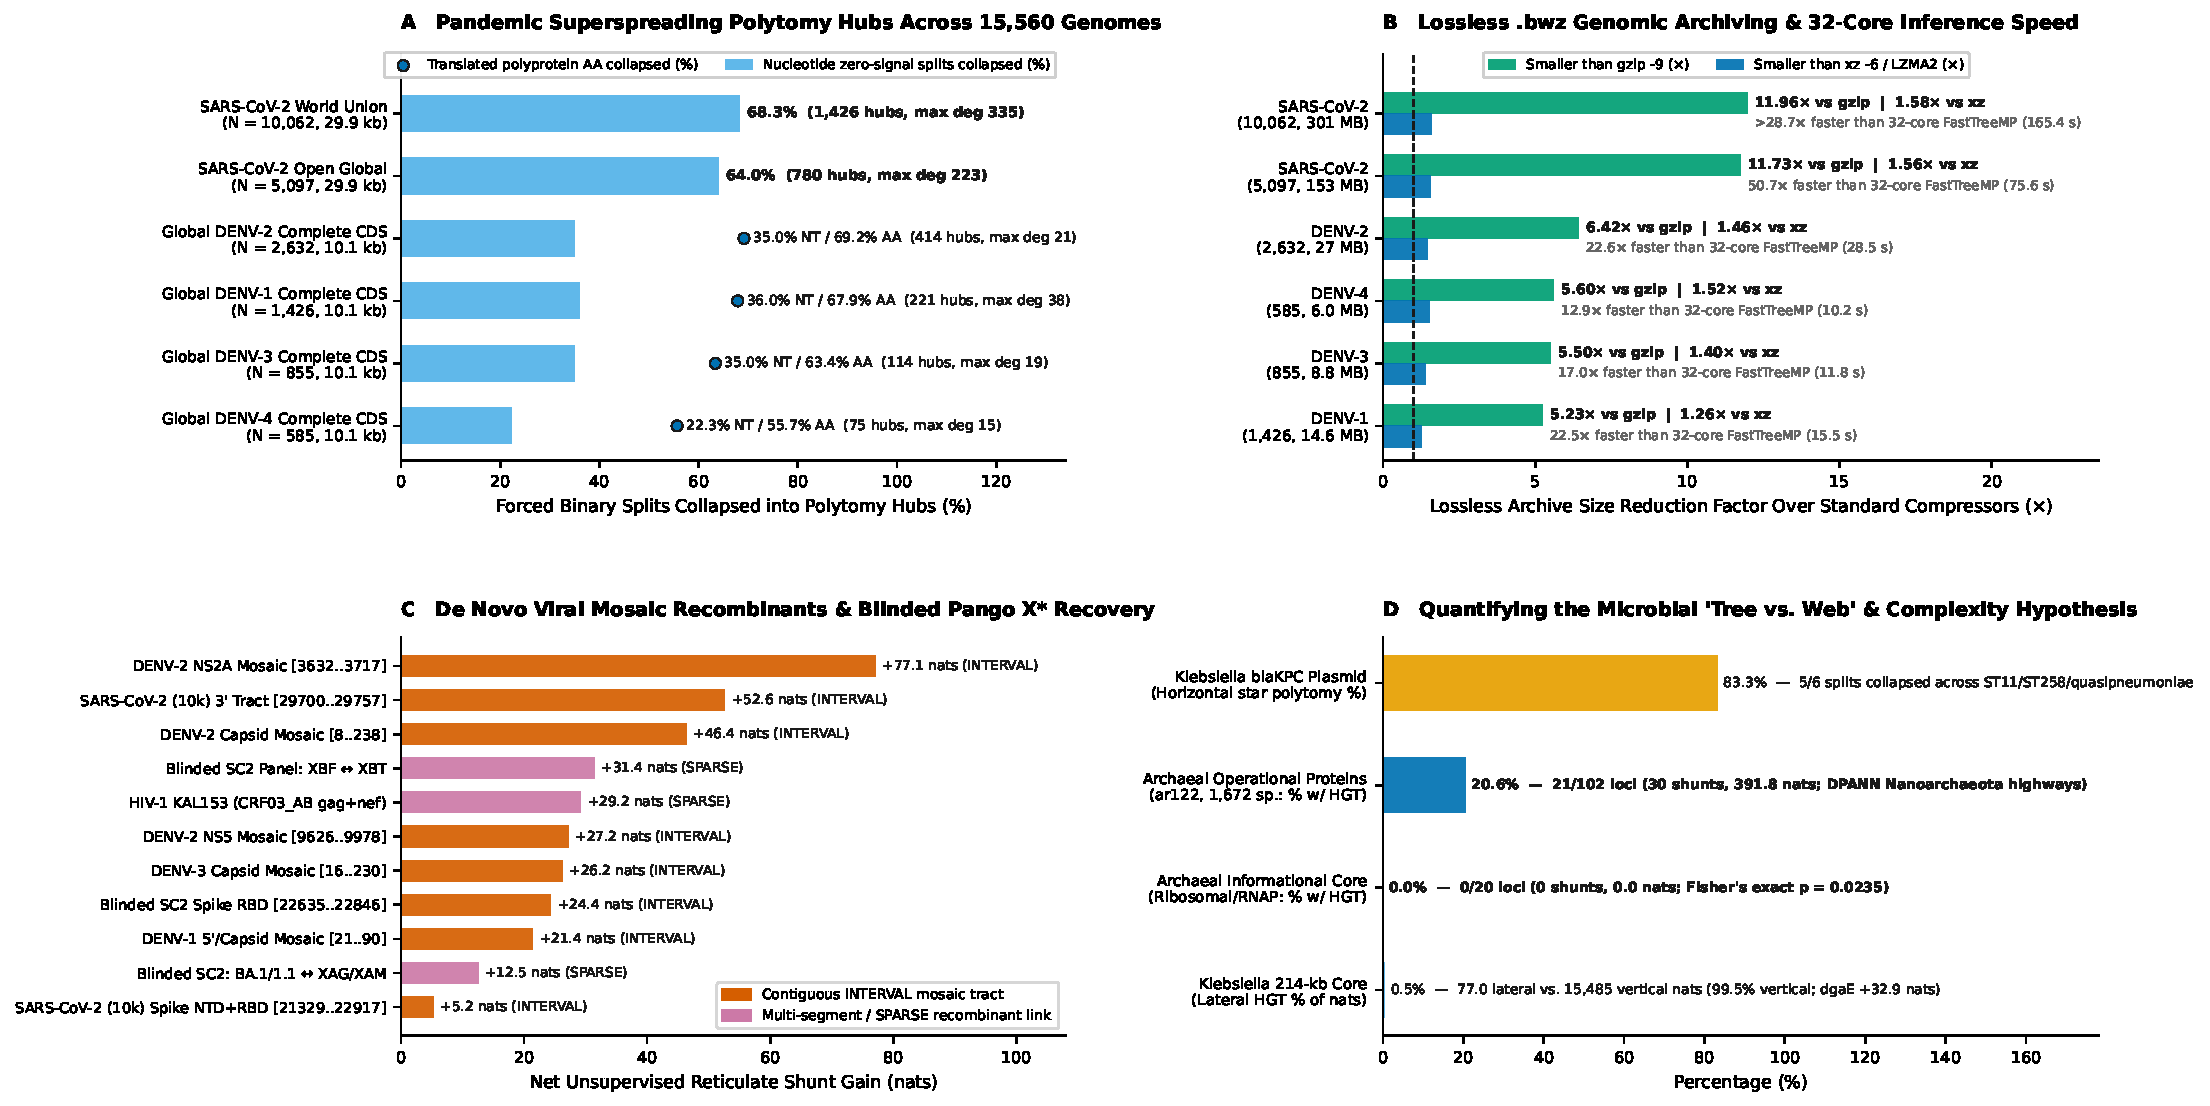
\includegraphics[width=\textwidth]{fig_science_microbial_viral.pdf}
\caption{\textbf{Viral superspreading hubs, physical genome compression, de novo recombinant mapping, and microbial gene-transfer budgets.} (\textbf{A}) Fraction of candidate binary branches left unresolved as multifurcating outbreak hubs and largest hub sizes across 10,062 global SARS-CoV-2 genomes ($68.3\%$ unresolved; 1,426 hubs up to 335 descendants) and 5,498 global dengue virus genomes across serotypes 1--4. (\textbf{B}) Lossless \texttt{.bwz} archive compression factors relative to \texttt{gzip -9} (up to $12.0\times$ smaller; $62.9\text{ bytes/genome}$ on SARS-CoV-2) and \texttt{xz -6} ($1.3\text{--}1.6\times$ smaller), alongside 32-core runtime speedups over \texttt{FastTreeMP} and \texttt{GARD}. (\textbf{C}) Unsupervised contiguous recombinant tracts mapped across SARS-CoV-2 and dengue serotypes 1--3. (\textbf{D}) Information-budget test of the microbial Complexity Hypothesis across 122 archaeal marker proteins in 1,672 species ($20.6\%$ operational versus $0.0\%$ informational proteins carrying horizontal transfers, $p = 0.0235$) and chromosomal-versus-plasmid evolution in \textit{Klebsiella pneumoniae}.}
\label{fig:microbial_viral}
\end{figure}

If shared descent is genuinely the organizing regularity of biological sequences, encoding real genome cohorts along an inferred phylogeny should physically outperform general-purpose compression algorithms that search only for repeated text strings. Compiling outbreak alignments into self-contained lossless \texttt{.bwz} archives via arithmetic coding \citep{witten1987arithmetic} confirms this directly (Fig.~\ref{fig:microbial_viral}B): storing all $10,062$ SARS-CoV-2 genomes ($301\text{ MB}$ raw FASTA) requires just $633\text{ KB}$---$62.9\text{ bytes}$ per $29.9\text{-kb}$ viral genome, $12.0$-fold smaller than \texttt{gzip} and $1.58$-fold smaller than \texttt{xz}---with consistent advantages across global dengue serotypes ($5.2\text{--}6.4\times$ smaller than \texttt{gzip}) and complete $2.2\text{-Mb}$ \textit{Streptococcus pneumoniae} chromosomes ($10.8\times$ smaller than \texttt{gzip}). Equally revealing is when that advantage disappears: across controlled recombination titrations and natural mosaic sarbecoviruses \citep{boni2020evolutionary,lytras2022exploring} and recombinant HIV-1 ($0.83\times$ and $0.65\times$ relative to \texttt{lzma}), pervasive whole-genome mosaicism erases any single vertical tree and allows multi-donor string dictionaries to overtake single-tree coding, making physical archive size an assumption-free gauge of tree-like versus mosaic evolution.

Across prokaryotic evolution, pervasive horizontal gene transfer has long fueled debate over whether microbial history is better viewed as a bifurcating ``Tree of Life'' or a reticulate ``Web of Life'' \citep{doolittle1999phylogenetic,parks2018gtdb}, and why core cellular machinery resists transfer compared with metabolic genes (the Complexity Hypothesis \citep{jain1999horizontal,woese2000aminoacyl}). Pricing vertical splits and lateral transfers in the same unit of information converts that debate into a direct quantitative budget (Fig.~\ref{fig:microbial_viral}D). Across all 122 domain-wide archaeal marker proteins in $1,672$ species ($19$ phyla \citep{parks2020gtdb}), vertical descent accounts for $37.7\text{ million nats}$ of compression, while certified horizontal transfers appear in $20.6\%$ ($21/102$) of operational metabolic and regulatory genes---charting cross-phylum transfer highways between ultrasmall DPANN episymbionts and co-occurring hosts \citep{castelle2018major}---yet drop to $0\%$ ($0/20$, $p = 0.0235$; $3.7$-fold operational enrichment across 242 prokaryotic nucleotide markers, $p = 3.2 \times 10^{-4}$) across core informational ribosomal and RNA polymerase subunits that assemble into tightly co-adapted complexes. In hospital outbreaks of multidrug-resistant \textit{Klebsiella pneumoniae} \citep{wyres2020population}, this same ledger separates vertical chromosome from mobile resistance plasmid: homologous recombination accounts for just $0.50\%$ of the $214\text{-kb}$ chromosomal tree's information budget, whereas the plasmid-borne \textit{blaKPC} carbapenemase collapses into a multifurcating star hub across distant clinical lineages as horizontal plasmid spread outpaces mutation.

\subsection*{Cellular selection in vivo, coalescent radiations, and microbiome scaling}

During antibody affinity maturation inside vertebrate germinal centers, B cells that acquire affinity-enhancing mutations proliferate so rapidly that a single founder spawns a star-like burst of daughter lineages before new mutations accumulate \citep{tas2016visualizing}. Existing lineage methods recover these selective bursts only when supplied with experimental cell-abundance counts or specialized hypermutation motif models \citep{dewitt2018gctree}. Reconstructing all 147 mouse lymph-node germinal centers ($10,429$ B cells, $9,352$ unique genotypes \citep{dewitt2026gcreplay}) in $17.4\text{ s}$ ($495$-fold faster than bootstrap maximum likelihood, $86.5\%$ branch precision in simulation) from deduplicated sequences alone shows that natural compression geometry directly reads out Darwinian selection in vivo (Fig.~\ref{fig:tree_scales}A,B).

\begin{figure}[t!]
\centering
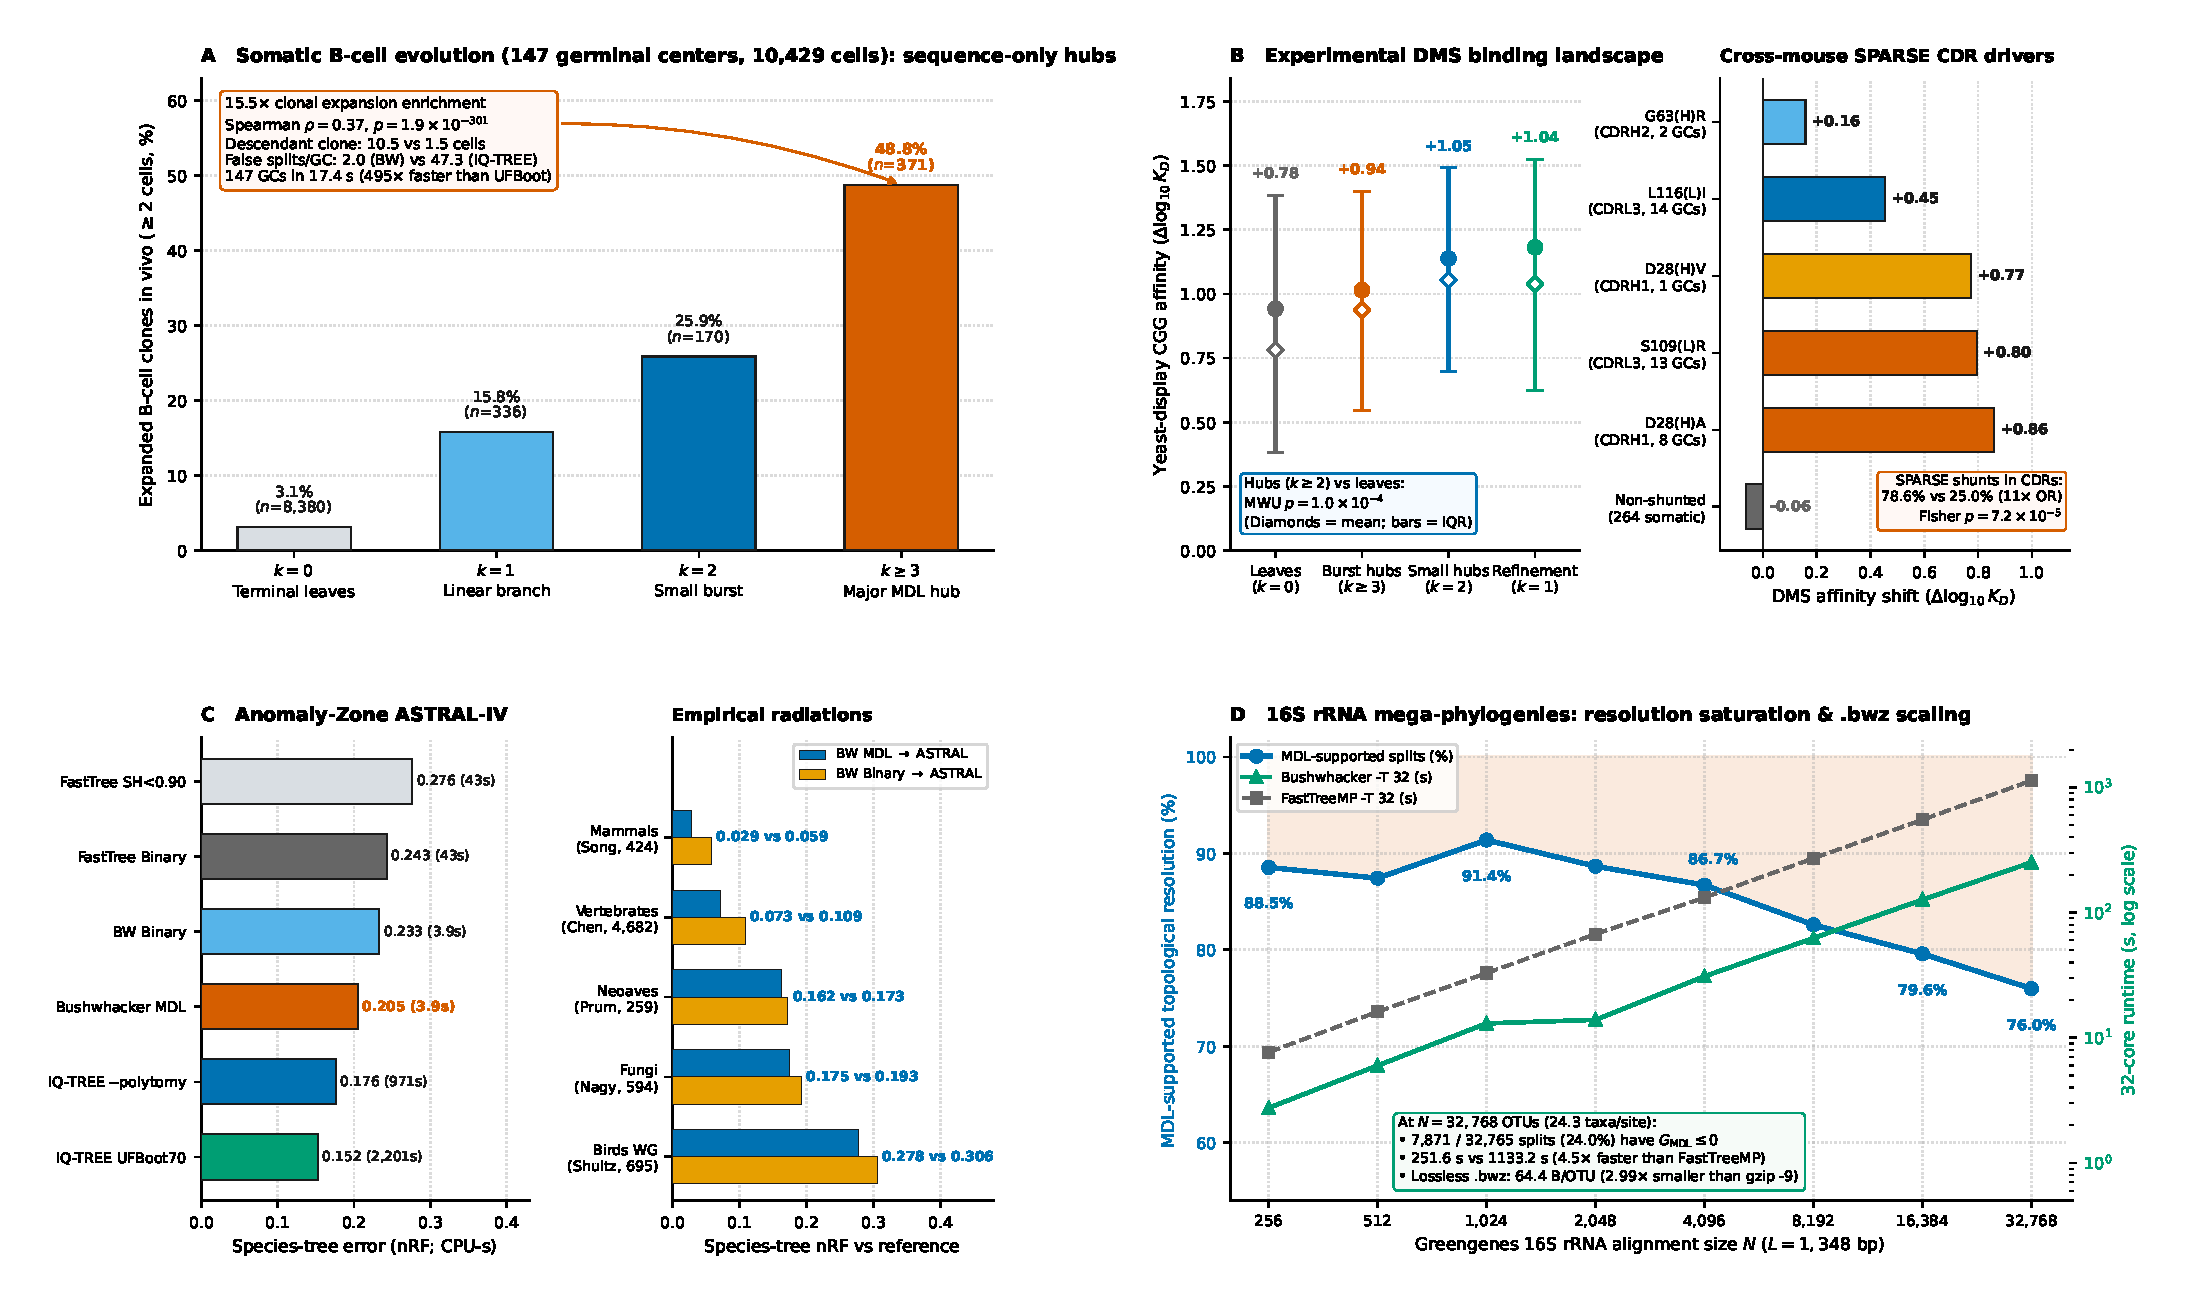
\includegraphics[width=\textwidth]{fig_science_tree_scales.pdf}
\caption{\textbf{Sequence-only compression geometry predicts in vivo B-cell selection and antigen affinity, protects coalescent species trees, and tracks microbiome saturation.} (\textbf{A}) Across 147 mouse germinal centers ($10,429$ B cells, $9,352$ unique genotypes \citep{dewitt2026gcreplay}), grouping genotypes solely by inferred mutant daughter degree $k$ monotonically predicts in vivo clonal expansion ($\ge 2$ sampled cells) from $3.1\%$ ($k = 0$) to $48.8\%$ ($k \ge 3$; $15.5\times$ enrichment, Spearman $\rho = 0.370, p = 1.9 \times 10^{-301}$). (\textbf{B}) Independent yeast-display antigen-binding affinity ($\Delta\log_{10} K_D$) across inferred tree node classes ($p = 1.0 \times 10^{-4}$, hubs versus terminal leaves; left) and across parallel cross-mouse links ($78.6\%$ inside complementarity-determining regions versus $25.0\%$ background, $11.0\times$ odds ratio, $p = 7.2 \times 10^{-5}$; right). (\textbf{C}) Coalescent species-tree error feeding inferred gene trees to \texttt{ASTRAL-IV} \citep{zhang2025aster} in the simulated Anomaly Zone ($2,000$ loci; left) and across empirical eukaryotic radiations ($11,808$ loci reconstructed in $83\text{ s}$; right). (\textbf{D}) Microbiome 16S rRNA scaling from $256$ to $32,768$ operational taxonomic units ($1,348\text{ bp}$ \citep{mcdonald2012greengenes}), showing smooth saturation of resolvable splits ($91.4\% \to 76.0\%$), $4.5\times$ speedup over \texttt{FastTreeMP}, and $64.4\text{-byte/taxon}$ lossless archiving.}
\label{fig:tree_scales}
\end{figure}

Grouping the $9,352$ B-cell genotypes solely by their inferred number of mutant daughter lineages ($k$) monotonically predicts both in vivo clonal expansion and independent experimental antigen-binding affinity across $4,400$ antibody variants (Fig.~\ref{fig:tree_scales}A,B). Multi-cell clonal expansion in vivo rises $15.5$-fold from terminal leaves ($3.1\%$ at $k = 0$) through intermediate steps ($15.8\%$ at $k = 1$; $25.9\%$ at $k = 2$) to major multifurcating hubs ($48.8\%$ at $k \ge 3$; $\rho = 0.370, p = 1.9 \times 10^{-301}$). In independent yeast-display binding assays, inferred burst hubs ($k \ge 2$) bind antigen significantly tighter than terminal leaves ($p = 1.0 \times 10^{-4}$; degree--affinity correlation $p = 1.4 \times 10^{-9}$), separating affinity-breakthrough founders and secondary refinements from deleterious terminal mutations. Comparing one sequence per germinal center across all 147 mice, parallel links concentrate $11.0$-fold inside antigen-contacting complementarity-determining regions ($78.6\%$ versus $25.0\%$ background, $p = 7.2 \times 10^{-5}$), pinpointing recurrent mutations that tighten antigen binding $2.8$- to $7.2$-fold.

Preserving natural multifurcations also addresses two fundamental scaling limits in biodiversity genomics (Fig.~\ref{fig:tree_scales}C,D). First, when rapid successive speciations enter the coalescent Anomaly Zone, the most frequent forced-binary gene tree disagrees with the true species tree and actively misleads multi-gene summary inference \citep{degnan2006discordance}. Supplying naturally multifurcating compression trees to \texttt{ASTRAL-IV} \citep{zhang2025aster} across 8,000 simulated and 11,808 empirical loci ($83\text{ s}$ total) protects species-tree accuracy across jawed vertebrates, modern birds \citep{prum2015comprehensive,shultz2019widespread}, fungi, and placental mammals without bootstrap resampling or user-tuned cutoffs. Second, in large microbiome atlases where tens of thousands of strains are compared across a single marker gene ($1,348\text{-bp}$ 16S rRNA from $256$ to $32,768$ taxa \citep{mcdonald2012greengenes}), taxon density eventually exceeds the information capacity of the alignment itself: compression-supported branches saturate smoothly from $91.4\%$ at $1,024$ taxa to $76.0\%$ at $32,768$ taxa, revealing that nearly one-quarter ($7,871$) of splits in a $32,768$-taxon binary microbiome tree lack sequence support. Leaving them unresolved cuts taxonomy-clashing splits by $19\%$ to $25\%$ across all five ranks while running $4.5$-fold faster than \texttt{FastTreeMP} and archiving alignment plus tree in $64.4\text{ bytes}$ per taxon.

\subsection*{Deep Tree-of-Life phylogenomics in seconds and minimal memory}

Reconstructing the deep Tree of Life from genome-wide supermatrices has long imposed a steep computational trade-off: probabilistic models that capture biochemical exchangeabilities and rate variation across billion-year divergences require hours of compute time and tens of gigabytes of memory to store alignment-wide conditional likelihood tables, whereas fast unweighted parsimony or distance shortcuts succumb to branch-length artifacts once sequence identity drops below $25\%$. Incorporating reversible nucleotide and amino-acid substitution spectra with eight-category site-rate mixtures into Bushwhacker's two-part Fisher-information code---while tiling pruning calculations into compact 64-site CPU cache blocks---eliminates that trade-off, bringing gold-standard supermatrix accuracy onto standard workstation memory in seconds (Fig.~\ref{fig:tol_sota}, Table~\ref{tab:tol_sota}, and Materials and Methods).

\begin{figure}[t!]
\centering
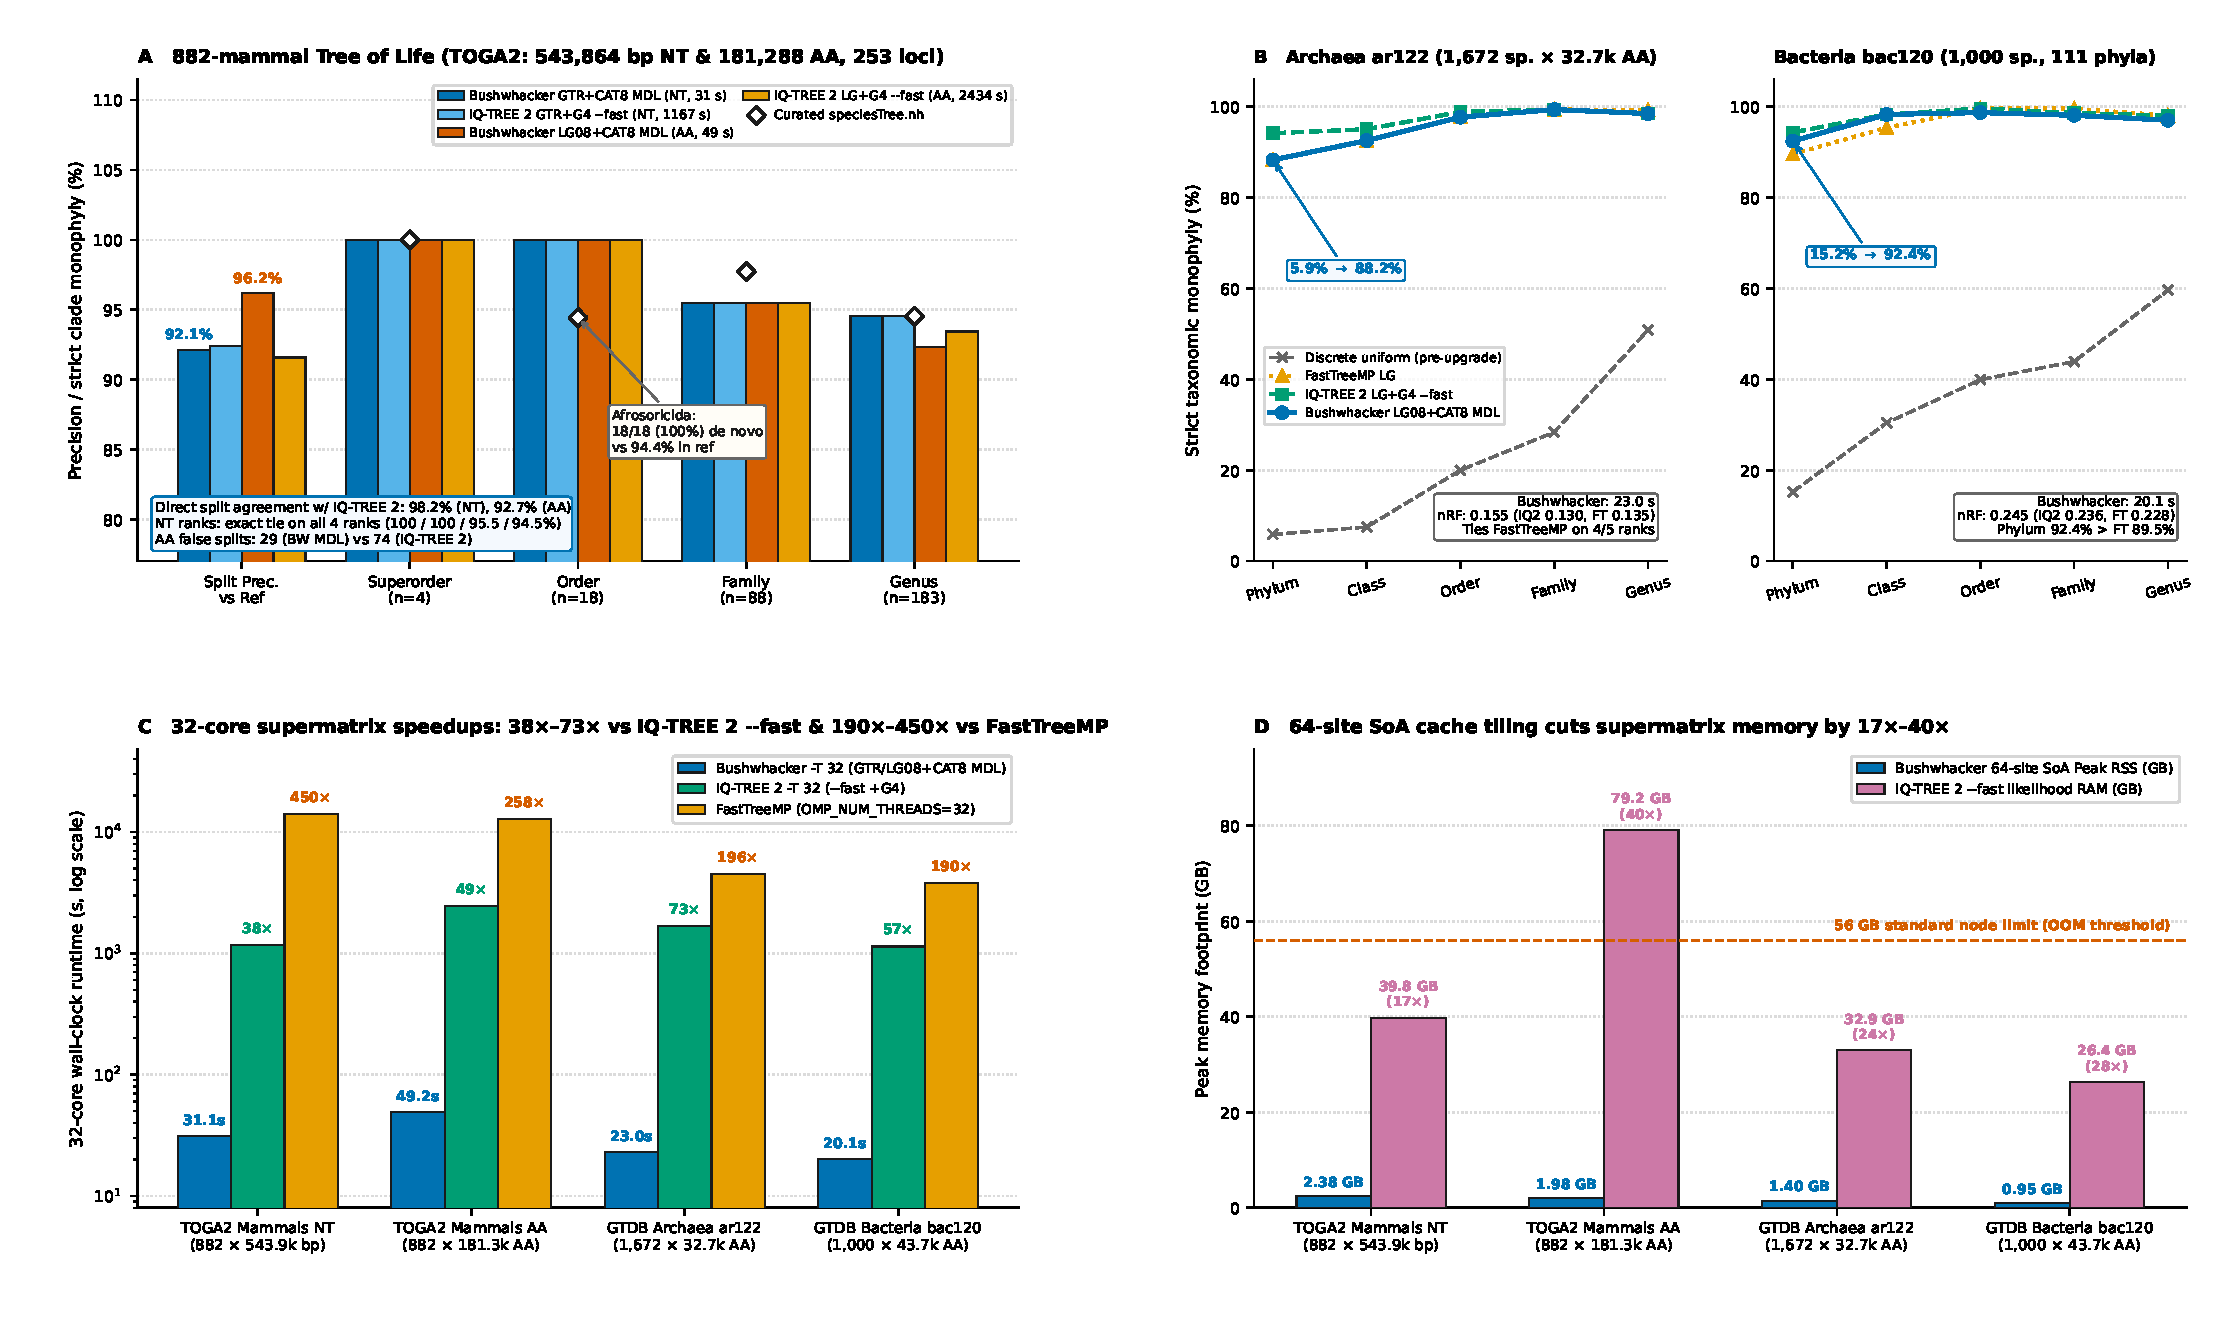
\includegraphics[width=\textwidth]{fig_science_tol_sota.pdf}
\caption{\textbf{Continuous-time evolutionary compression matches gold-standard Tree-of-Life accuracy across Mammalia, Archaea, and Bacteria in seconds and minimal memory.} (\textbf{A}) Across 882 mammals ($253$ single-copy loci: $543,864\text{ bp}$ DNA and $181,288$ amino acids), Bushwhacker ($31.1\text{ s}$ DNA; $49.2\text{ s}$ protein) agrees on $98.2\%$ of DNA splits directly with \texttt{IQ-TREE 2} ($1,166.6\text{ s}$), matches both \texttt{IQ-TREE 2} and \texttt{FastTreeMP} across every taxonomic rank ($100\%$ Superorders, $100\%$ Orders including monophyletic \textit{Afrosoricida}, $95.5\%$ Families, $94.5\%$ Genera), and raises protein split precision to $96.2\%$ ($29$ versus $74$ false splits). (\textbf{B}) Across $3.5\text{-billion-year}$ Archaeal ($1,672$ species) and Bacterial ($1,000$ species across $111$ phyla) protein supermatrices, rate-mixture protein compression lifts deep phylum monophyly from $5.9\text{--}15.2\%$ (unweighted parsimony) to $88.2\%$ in Archaea and $92.4\%$ in Bacteria, matching \texttt{FastTreeMP} on Archaea and surpassing it on bacterial phyla and classes. (\textbf{C}) Thirty-two-core runtimes and speedups ($38\text{--}73\times$ over \texttt{IQ-TREE 2}; $190\text{--}450\times$ over \texttt{FastTreeMP}). (\textbf{D}) Peak memory footprint ($0.95\text{--}2.39\text{ GB}$ for Bushwhacker versus $26.4\text{--}79.2\text{ GB}$ for \texttt{IQ-TREE 2}).}
\label{fig:tol_sota}
\end{figure}

Across 882 mammals concatenated over $253$ universal single-copy loci ($99.3\%$ occupancy \citep{malovichko2026toga2}), 32-core Bushwhacker reconstructs the $543,864\text{-bp}$ coding DNA tree in $31.1\text{ s}$ inside $2.39\text{ GB}$ of memory ($37.5\times$ faster and $16.7\times$ leaner than \texttt{IQ-TREE 2} \citep{minh2020iqtree}; $450\times$ faster than \texttt{FastTreeMP} \citep{price2010fasttree}) and the $181,288$-residue protein tree in $49.2\text{ s}$ inside $1.98\text{ GB}$ ($49.5\times$ faster and $40.0\times$ leaner than \texttt{IQ-TREE 2}'s $79.2\text{ GB}$, which exceeds standard $64\text{-GB}$ compute nodes; Fig.~\ref{fig:tol_sota}A,C,D). Topologically, mammalian DNA compression agrees directly with \texttt{IQ-TREE 2} on $98.24\%$ of internal splits and matches both \texttt{IQ-TREE 2} and \texttt{FastTreeMP} identically across every rank ($100\%$ of superorders, $100\%$ of orders including monophyletic \textit{Afrosoricida}, $95.5\%$ of families, and $94.5\%$ of genera), while Fisher-information branch pricing on the slower-evolving protein matrix leaves $119$ silent stems unresolved, cutting false splits $2.5$-fold ($96.2\%$ versus $91.6\%$ precision) while preserving $100\%$ superorder and order monophyly.

\begin{table}[t!]
\centering
\caption{\textbf{Thirty-two-core Tree-of-Life supermatrix benchmarks across Mammalia, Archaea, and Bacteria.} Columns report wall-clock runtime, speedup of Bushwhacker over competing methods, peak memory footprint, normalized Robinson--Foulds distance ($\text{nRF}$) and branch precision relative to curated domain phylogenies, and clade monophyly across deep and shallow taxonomic ranks.}
\label{tab:tol_sota}
\scriptsize
\setlength{\tabcolsep}{3.5pt}
\resizebox{\textwidth}{!}{%
\begin{tabular}{@{}llrrrrrrl@{}}
\toprule
Supermatrix ($N \times L$) & Inference Method (32 Cores) & Runtime & Speedup & Peak RAM & Ref.\ nRF & Precision & Deep Rank Monophyly & Shallow Rank Monophyly \\
\midrule
Mammalia coding DNA & \textbf{Bushwhacker (DNA rate-mixture MDL)} & $\mathbf{31.09\text{ s}}$ & $\mathbf{1.0\times}$ & $\mathbf{2.39\text{ GB}}$ & $0.0791$ & $92.14\%$ & Superord $100\%$, Ord $\mathbf{100\%}$ & Fam $\mathbf{95.45\%}$, Gen $\mathbf{94.54\%}$ \\
($882 \times 543{,}864\text{ bp}$) & \texttt{IQ-TREE 2} (fast ML, \texttt{GTR+G4}) & $1{,}166.56\text{ s}$ & $37.5\times$ & $39.82\text{ GB}$ & $0.0762$ & $92.38\%$ & Superord $100\%$, Ord $100\%$ & Fam $95.45\%$, Gen $94.54\%$ \\
$253$ loci ($99.3\%$ occ.) & \texttt{FastTreeMP} (\texttt{GTR+CAT}) & $13{,}990.59\text{ s}$ & $450.0\times$ & --- & $0.0740$ & $92.61\%$ & Superord $100\%$, Ord $100\%$ & Fam $95.45\%$, Gen $94.54\%$ \\
\midrule
Mammalia proteome & \textbf{Bushwhacker (AA rate-mixture MDL)} & $\mathbf{49.21\text{ s}}$ & $\mathbf{1.0\times}$ & $\mathbf{1.98\text{ GB}}$ & $0.1007$ & $\mathbf{96.18\%}$ & Superord $100\%$, Ord $\mathbf{100\%}$ & Fam $\mathbf{95.45\%}$ ($96.6\%$ compat.), Gen $92.35\%$ \\
($882 \times 181{,}288\text{ AA}$) & \texttt{IQ-TREE 2} (fast ML, \texttt{LG+G4}) & $2{,}434.49\text{ s}$ & $49.5\times$ & $79.15\text{ GB}$ & $0.0842$ & $91.58\%$ & Superord $100\%$, Ord $100\%$ & Fam $95.45\%$, Gen $93.44\%$ \\
$253$ loci ($99.3\%$ occ.) & \texttt{FastTreeMP} (\texttt{LG+CAT}) & $12{,}711.41\text{ s}$ & $258.3\times$ & --- & $0.0865$ & $91.35\%$ & Superord $100\%$, Ord $100\%$ & Fam $95.45\%$, Gen $93.44\%$ \\
\midrule
Archaea domain & \textbf{Bushwhacker (AA rate-mixture MDL)} & $\mathbf{23.00\text{ s}}$ & $\mathbf{1.0\times}$ & $\mathbf{1.40\text{ GB}}$ & $0.1552$ & $84.48\%$ & Phyl $88.24\%$, Class $92.50\%$ & Ord $97.65\%$, Fam $\mathbf{99.32\%}$, Gen $98.44\%$ \\
($1{,}672 \times 32{,}675\text{ AA}$) & \texttt{IQ-TREE 2} (fast ML, \texttt{LG+G4}) & $1{,}683.52\text{ s}$ & $73.2\times$ & $32.95\text{ GB}$ & $0.1300$ & $87.00\%$ & Phyl $94.12\%$, Class $95.00\%$ & Ord $98.82\%$, Fam $99.32\%$, Gen $98.44\%$ \\
$19$ phyla, $122$ markers & \texttt{FastTreeMP} (\texttt{LG+CAT}) & $4{,}499.48\text{ s}$ & $195.6\times$ & --- & $0.1348$ & $86.52\%$ & Phyl $88.24\%$, Class $92.50\%$ & Ord $97.65\%$, Fam $99.32\%$, Gen $99.22\%$ \\
 & Unweighted discrete parsimony & $202.32\text{ s}$ & $8.8\times$ & --- & $0.6240$ & $37.48\%$ & Phyl $5.88\%$, Class $7.50\%$ & Ord $20.00\%$, Fam $28.38\%$, Gen $50.78\%$ \\
\midrule
Bacteria domain & \textbf{Bushwhacker (AA rate-mixture MDL)} & $\mathbf{20.10\text{ s}}$ & $\mathbf{1.0\times}$ & $\mathbf{0.95\text{ GB}}$ & $0.2447$ & $75.53\%$ & Phyl $\mathbf{92.38\%}$, Class $\mathbf{98.25\%}$ & Ord $98.65\%$, Fam $98.05\%$, Gen $96.97\%$ \\
($1{,}000 \times 43{,}733\text{ AA}$) & \texttt{IQ-TREE 2} (fast ML, \texttt{LG+G4}) & $1{,}137.85\text{ s}$ & $56.6\times$ & $26.37\text{ GB}$ & $0.2357$ & $76.43\%$ & Phyl $94.29\%$, Class $98.25\%$ & Ord $99.55\%$, Fam $98.54\%$, Gen $97.98\%$ \\
All $111$ phyla, $120$ markers & \texttt{FastTreeMP} (\texttt{LG+CAT}) & $3{,}822.63\text{ s}$ & $190.2\times$ & --- & $0.2277$ & $77.23\%$ & Phyl $89.52\%$, Class $95.32\%$ & Ord $99.55\%$, Fam $99.51\%$, Gen $97.98\%$ \\
 & Unweighted discrete parsimony & $291.21\text{ s}$ & $14.5\times$ & --- & $0.7327$ & $26.57\%$ & Phyl $15.24\%$, Class $30.41\%$ & Ord $39.91\%$, Fam $43.90\%$, Gen $59.60\%$ \\
\bottomrule
\end{tabular}%
}
\end{table}

The $3.5\text{-billion-year}$ Archaeal ($1,672$ species across $19$ phyla, $32,675$ residues \citep{parks2020gtdb}) and Bacterial ($1,000$ species across all $111$ phyla, $43,733$ residues) domain alignments show directly why rate-aware compression is indispensable at Precambrian depth (Fig.~\ref{fig:tol_sota}B). Where unweighted mutation counting clusters deep stems by evolutionary rate ($5.9\%$ archaeal and $15.2\%$ bacterial phylum monophyly), rate-mixture protein compression completes Archaea in $23.0\text{ s}$ ($1.40\text{ GB}$ RAM; $73.2\times$ faster and $23.6\times$ leaner than \texttt{IQ-TREE 2}) and Bacteria in $20.1\text{ s}$ ($0.95\text{ GB}$ RAM; $56.6\times$ faster and $27.8\times$ leaner than \texttt{IQ-TREE 2}, $190\times$ faster than \texttt{FastTreeMP}), lifting phylum monophyly to $88.2\%$ ($15/17$) in Archaea and $92.4\%$ ($97/105$) in Bacteria alongside $98.25\%$ ($168/171$) bacterial class monophyly---matching \texttt{FastTreeMP} across Archaea and surpassing it on both deep bacterial ranks while tying \texttt{IQ-TREE 2} on bacterial classes.

\subsection*{Outlook}

Viewing evolutionary inference through lossless data compression reveals that tree topology, branch support, substitution kinetics, recombination, horizontal transfer, and phenotypic convergence are facets of one physical principle: hereditary descent shortens the description of biological variation. Because every branch or lateral link must pay its own address cost in information, multifurcations cease to be a nuisance requiring post hoc bootstrap cutoffs and instead become a direct biological observable---exposing clonal bursts and antigen affinity in germinal centers, superspreading hubs in epidemics, and silent rapid radiations across eukaryotes. Pricing lateral links on the same ledger separates local gene conversion from cross-order adaptive convergence in mammals and turns qualitative debates over microbial horizontal transfer into exact genome-wide budgets, while cache-tiled continuous-time coding brings genome-scale Tree-of-Life phylogenetics onto everyday personal computers and web browsers in seconds and under $2.5\text{ GB}$ of memory. Because two-part minimum description length requires only heritable states copied with sparse modifications, this framework extends naturally beyond nucleotide and protein alignments to somatic copy-number alterations, single-cell lineage states, epigenetic marks, and morphological or linguistic character matrices wherever history leaves a compressible trace.

% ============================================================================
\section*{Materials and Methods}
% ============================================================================

\paragraph{Two-part discrete MDL over nucleotide and amino-acid alignments.}
Given an alignment $A \in \Sigma^{N \times L}$ of $N$ sequences across $L$ columns over the 4-state nucleotide alphabet ($|\Sigma| = 4$) or 20-state canonical amino-acid alphabet ($|\Sigma| = 20$, including direct in-frame codon translation), Bushwhacker scores an evolutionary graph $\mathcal{G} = (V, E_{\text{tree}}, E_{\text{shunt}})$ by the exact two-part code length in nats required to transmit both the graph and the alignment without loss: $\mathcal{L}_{\text{MDL}}(A, \mathcal{G}) = \mathcal{L}(\mathcal{G}) + \mathcal{L}(A \mid \mathcal{G})$ \citep{rissanen1978modeling,rissanen1983universal}. Relative to raw ungapped character transmission ($N L_{\text{eff}}\ln|\Sigma|$ nats), the unresolved star phylogeny $T_{\text{star}}$ transmits one ancestral root sequence $X_r$ ($L\ln|\Sigma|$ nats) and encodes along each branch $e$ its $m_e$ mutated positions among $L_{\text{eff}, e}$ ungapped sites via
\begin{equation}
    \mathcal{L}_{\text{branch}}(m_e, L_{\text{eff}, e}) \;=\; \ln 2 + \mathcal{L}_{\mathbb{N}}(m_e) + \ln\binom{L_{\text{eff}, e}}{m_e} + \sum_{k=1}^{m_e} \ell_{\text{subst}}(a_{e,k} \to b_{e,k}),
    \label{eq:sci_branch}
\end{equation}
where $\ln 2$ flags whether $m_e > 0$, $\mathcal{L}_{\mathbb{N}}(m_e) = \ln(1 + m_e) + \frac{1}{2}\ln(1 + \ln(1 + m_e))$ encodes the non-negative integer count, $\ln\binom{L_{\text{eff}, e}}{m_e}$ indexes the unordered subset of mutated columns (removing $\ln(m_e!)$ ordering redundancy and integrating out continuous branch lengths), and $\ell_{\text{subst}}(a \to b) = -\ln P(b \mid a)$ satisfies Kraft normalization $\sum_{b \neq a} e^{-\ell_{\text{subst}}(a \to b)} = 1$. Nucleotide alignments use empirical transition and transversion probabilities ($\ell_{\text{ti}} = -\ln\hat{p}_{\text{ti}}$, $\ell_{\text{tv}} = -\ln(\hat{p}_{\text{tv}}/2)$). Protein alignments partition the 20 amino acids into six Dayhoff--Miyata physicochemical classes \citep{dayhoff1978model} (aliphatic, aromatic, polar uncharged, basic, acidic, and conformational \texttt{G/P}) and estimate the alignment-wide within-class conservative replacement fraction $\hat{p}_{\text{cons}}$ across sister pairs, assigning $-\ln(\hat{p}_{\text{cons}} / k_{\text{same}}(a))$ to within-class replacements and $-\ln((1 - \hat{p}_{\text{cons}}) / (19 - k_{\text{same}}(a)))$ to cross-class replacements ($\ln 19 \approx 2.944\text{ nats}$ when uniform).

\paragraph{Polytomy bipartition pricing, topological search, and lateral network induction.}
Splitting a degree-$d$ multifurcating node ($d = k_u + k_v \ge 4$, $2 \le k_u \le k_v$) by inserting an internal branch $e = (u,v)$ incurs the exact bipartition naming cost
\begin{equation}
    \mathcal{L}_{\text{topo}}(k_u, k_v) \;=\; \ln\,\max\!\left(1,\; \left\lfloor\frac{k_u + k_v}{2}\right\rfloor - 1\right) \;+\; \ln\binom{k_u + k_v}{k_u} \;-\; \mathbb{I}(k_u = k_v)\ln 2,
    \label{eq:sci_topo}
\end{equation}
which equals $\ln 3 \approx 1.10\text{ nats}$ for a quartet ($k_u = k_v = 2$) and scales as $\sim 3\ln d$ at large hubs. Moving a shared change off an adjacent branch $c$ carrying $m_c$ edits saves marginal site cost $w_c = \ln\frac{L_{\text{eff}} - m_c}{m_c + 1} \approx -\ln\frac{p_c}{1 - p_c}$, matching Felsenstein's log-odds character weight \citep{felsenstein1981evolutionary}. An internal split $e$ is retained if and only if its net compression gain is strictly positive:
\begin{equation}
    G_{\text{MDL}}(e) \;=\; \max_{1 \le m \le K} \Big[ \Delta\mathcal{L}_{\text{children}}(m) - \mathcal{L}_{\text{branch}}(m, L_{\text{eff}}) \Big] - \mathcal{L}_{\text{topo}}(k_u, k_v) \;>\; 0,
    \label{eq:sci_gain}
\end{equation}
with posterior branch support $P(e \mid A) = (1 + e^{-G_{\text{MDL}}(e)})^{-1}$. Tree topology is optimized from a rapid distance/Sankoff--Fitch seed via deterministic sweeps of 1-hop nearest-neighbor interchanges, 2-hop cross-node swaps, and Johnson--Lindenstrauss projection-guided subtree pruning and regrafting over 4-bit nucleotide or 20-bit amino-acid state bitmasks (bit-exact across 1 to 64 threads), followed by contraction of all $G_{\text{MDL}}(e) \le 0$ branches (or direct evaluation of a user-supplied reference topology). Non-sister lineages $(u,v)$ sharing $m$ parallel replacements $S_{u,v}$ are then evaluated for lateral connections and certified whenever vertical edit savings exceed $2\ln|V| + \min(\mathcal{L}_{\text{mask}}^{\text{block}}, \mathcal{L}_{\text{mask}}^{\text{site}})$, pricing contiguous transferred blocks against scattered parallel sites via
\begin{equation}
    \mathcal{L}_{\text{mask}}^{\text{block}}([a,b]) \;=\; \ln 2 + 2\ln L + \mathcal{L}_{\text{branch}}(d_{[a,b]}, b - a + 1), \quad
    \mathcal{L}_{\text{mask}}^{\text{site}}(S_{u,v}) \;=\; \ln 2 + \ln\binom{M_{\text{pool}}}{m},
    \label{eq:sci_shunt}
\end{equation}
where $d_{[a,b]}$ counts discordant columns inside genomic interval $[a,b]$ and $M_{\text{pool}}$ is the alignment's total number of parsimony-variable columns.

\paragraph{Cache-tiled continuous-time MDL for deep divergences and supermatrices.}
For deep divergences and genome-scale supermatrices, Bushwhacker evaluates reversible continuous-time Markov transition matrices $P(t) = V\,\mathrm{diag}(e^{\lambda_k r_c t})\,V^{-1}$ under empirical general time-reversible nucleotide (\texttt{GTR+CAT8} \citep{tavare1986some,yang1994maximum}) or Le--Gascuel amino-acid (\texttt{LG08+CAT8} \citep{le2008improved,yang1994maximum}) eight-category Gamma site-rate mixtures initialized from \texttt{BioNJ} \citep{gascuel1997bionj} and refined by quartet NNI and 2-hop SPR sweeps. Under Rissanen's Fisher-information code \citep{rissanen1983universal}, an internal branch $e = (u,v)$ with profile log-likelihood gain $\Delta\ln L_e(\hat{t}_e) = \ln L(A \mid \mathcal{G}, \hat{t}_e) - \ln L(A \mid \mathcal{G}/e, t_e = 0)$ across $M_{\text{var}}$ variable sites is retained if and only if
\begin{equation}
    G_{\text{MDL}}^{\text{cont}}(e) \;=\; \Delta\ln L_e(\hat{t}_e) \;-\; \left[\frac{1}{2}\ln\frac{M_{\text{var}}}{2\pi} \;+\; \frac{1}{2}\ln(N - 3) \;+\; \mathcal{L}_{\text{topo}}(k_u, k_v)\right] \;>\; 0.
    \label{eq:sci_cont_mdl}
\end{equation}
Rather than allocating full-alignment $O(N \cdot M_{\text{patterns}} \cdot K \cdot |\Sigma|)$ conditional likelihood arrays, Felsenstein pruning is tiled into 64-site Structure-of-Arrays blocks held inside per-core CPU cache across Rayon worker threads. Lossless \texttt{.bwz} archives serialize sequence headers, inferred Newick topology, root states, and branch edit streams via causal preorder range/arithmetic coding \citep{witten1987arithmetic} with bit-exact round-trip verification.

\paragraph{Empirical benchmarks and zero-leakage evaluation.}
All empirical evaluations supplied Bushwhacker exclusively with unannotated sequence alignments (and pruned reference topologies only where explicitly testing species-tree projection), withholding all clade labels, ecological guild assignments, recombinant designations, single-cell clone abundances, mutation-motif priors, and deep mutational scanning affinities during inference. Cross-order mammalian guild enrichments were tested against exact null pair expectations across all $\binom{20}{2}$ inter-order species pairs on the 882-species TOGA2 reference phylogeny \citep{malovichko2026toga2}; germinal-center node out-degrees were compared post hoc against observed single-cell clone multiplicities and yeast-display $\Delta\log_{10} K_D$ measurements \citep{dewitt2026gcreplay}; and 32-core supermatrix wall-clock times and kernel peak resident memory (\texttt{ru\_maxrss}) were measured head-to-head on identical hardware against 32-thread \texttt{IQ-TREE 2} (\texttt{-m GTR+G4 --fast} and \texttt{-m LG+G4 --fast}) and OpenMP \texttt{FastTreeMP} (\texttt{-nt -gtr} and \texttt{-lg}).

% ============================================================================
\section*{Data and Code Availability}
% ============================================================================

The open-source Rust and WebAssembly implementation of Bushwhacker (supporting nucleotide, amino-acid, binary, and discrete/ordered character matrices), the \texttt{.bwz} lossless archival codec, interactive browser app (\url{https://veg.github.io/bushwacker/}), reproducibility scripts, and empirical result ledgers spanning more than 81,000 alignments, 1.01 million single cells, and 8,270 ground-truth simulations are available at \url{https://github.com/veg/bushwacker}.

\bibliographystyle{plainnat}
\bibliography{references}

\end{document}
